\documentclass[preprint, 3p,
authoryear]{elsarticle} %review=doublespace preprint=single 5p=2 column
%%% Begin My package additions %%%%%%%%%%%%%%%%%%%

\usepackage[hyphens]{url}


\usepackage{graphicx}
%%%%%%%%%%%%%%%% end my additions to header

\usepackage[T1]{fontenc}
\usepackage{lmodern}
\usepackage{amssymb,amsmath}
% TODO: Currently lineno needs to be loaded after amsmath because of conflict
% https://github.com/latex-lineno/lineno/issues/5
\usepackage{lineno} % add
  \linenumbers % turns line numbering on
\usepackage{ifxetex,ifluatex}
\usepackage{fixltx2e} % provides \textsubscript
% use upquote if available, for straight quotes in verbatim environments
\IfFileExists{upquote.sty}{\usepackage{upquote}}{}
\ifnum 0\ifxetex 1\fi\ifluatex 1\fi=0 % if pdftex
  \usepackage[utf8]{inputenc}
\else % if luatex or xelatex
  \usepackage{fontspec}
  \ifxetex
    \usepackage{xltxtra,xunicode}
  \fi
  \defaultfontfeatures{Mapping=tex-text,Scale=MatchLowercase}
  \newcommand{\euro}{€}
\fi
% use microtype if available
\IfFileExists{microtype.sty}{\usepackage{microtype}}{}

\ifxetex
  \usepackage[setpagesize=false, % page size defined by xetex
              unicode=false, % unicode breaks when used with xetex
              xetex]{hyperref}
\else
  \usepackage[unicode=true]{hyperref}
\fi
\hypersetup{breaklinks=true,
            bookmarks=true,
            pdfauthor={},
            pdftitle={The complex network of trophic interactions in a subAntarctic oceanic Marine Protected Area},
            colorlinks=false,
            urlcolor=blue,
            linkcolor=magenta,
            pdfborder={0 0 0}}

\setcounter{secnumdepth}{5}
% Pandoc toggle for numbering sections (defaults to be off)


% tightlist command for lists without linebreak
\providecommand{\tightlist}{%
  \setlength{\itemsep}{0pt}\setlength{\parskip}{0pt}}

% From pandoc table feature
\usepackage{longtable,booktabs,array}
\usepackage{calc} % for calculating minipage widths
% Correct order of tables after \paragraph or \subparagraph
\usepackage{etoolbox}
\makeatletter
\patchcmd\longtable{\par}{\if@noskipsec\mbox{}\fi\par}{}{}
\makeatother
% Allow footnotes in longtable head/foot
\IfFileExists{footnotehyper.sty}{\usepackage{footnotehyper}}{\usepackage{footnote}}
\makesavenoteenv{longtable}

% Pandoc citation processing
\newlength{\cslhangindent}
\setlength{\cslhangindent}{1.5em}
\newlength{\csllabelwidth}
\setlength{\csllabelwidth}{3em}
\newlength{\cslentryspacingunit} % times entry-spacing
\setlength{\cslentryspacingunit}{\parskip}
% for Pandoc 2.8 to 2.10.1
\newenvironment{cslreferences}%
  {}%
  {\par}
% For Pandoc 2.11+
\newenvironment{CSLReferences}[2] % #1 hanging-ident, #2 entry spacing
 {% don't indent paragraphs
  \setlength{\parindent}{0pt}
  % turn on hanging indent if param 1 is 1
  \ifodd #1
  \let\oldpar\par
  \def\par{\hangindent=\cslhangindent\oldpar}
  \fi
  % set entry spacing
  \setlength{\parskip}{#2\cslentryspacingunit}
 }%
 {}
\usepackage{calc}
\newcommand{\CSLBlock}[1]{#1\hfill\break}
\newcommand{\CSLLeftMargin}[1]{\parbox[t]{\csllabelwidth}{#1}}
\newcommand{\CSLRightInline}[1]{\parbox[t]{\linewidth - \csllabelwidth}{#1}\break}
\newcommand{\CSLIndent}[1]{\hspace{\cslhangindent}#1}


\usepackage{booktabs}
\usepackage{longtable}
\usepackage{array}
\usepackage{multirow}
\usepackage{wrapfig}
\usepackage{float}
\usepackage{colortbl}
\usepackage{pdflscape}
\usepackage{tabu}
\usepackage{threeparttable}
\usepackage{threeparttablex}
\usepackage[normalem]{ulem}
\usepackage{makecell}
\usepackage{xcolor}



\begin{document}


\begin{frontmatter}

  \title{The complex network of trophic interactions in a subAntarctic
oceanic Marine Protected Area}
    \author[]{Tomás I. Marina\textsuperscript{a}%
  \corref{cor1}%
  }
   \ead{tomasimarina@gmail.com} 
    \author[]{Irene R. Schloss\textsuperscript{a,b,c}%
  %
  }
  
    \author[]{Gustavo A. Lovrich\textsuperscript{a}%
  %
  }
  
    \author[]{Claudia C. Boy\textsuperscript{a}%
  %
  }
  
    \author[]{Daniel O. Bruno\textsuperscript{a,c}%
  %
  }
  
    \author[]{Fabiana L. Capitanio\textsuperscript{d,e}%
  %
  }
  
    \author[]{Sergio M. Delpiani\textsuperscript{f}%
  %
  }
  
    \author[]{Juan Martín Díaz de Astarloa\textsuperscript{f}%
  %
  }
  
    \author[]{Cintia Fraysse\textsuperscript{a}%
  %
  }
  
    \author[]{Virginia A. García Alonso\textsuperscript{d,e}%
  %
  }
  
    \author[]{Andrea Raya Rey\textsuperscript{a,c,g}%
  %
  }
  
    \author[]{Laura Schejter\textsuperscript{h}%
  %
  }
  
    \author[]{Mariela L. Spinelli\textsuperscript{d,e}%
  %
  }
  
    \author[]{Marcos Tatián\textsuperscript{i,j}%
  %
  }
  
    \author[]{Diego Urteaga\textsuperscript{k}%
  %
  }
  
    \author[]{Luciana Riccialdelli\textsuperscript{a}%
  %
  }
  
      \affiliation[1]{Centro Austral de Investigaciones Científicas
(CADIC-CONICET), Ushuaia, Argentina}
    \affiliation[2]{Instituto Antártico Argentino (IAA), CABA,
Argentina}
    \affiliation[3]{Instituto de Ciencias Polares, Ambiente y Recursos
Naturales (ICPA), Universidad de Tierra del Fuego (UNTDF), Ushuaia,
Argentina}
    \affiliation[4]{Facultad de Ciencias Exactas y Naturales,
Universidad de Buenos Aires (UBA), CABA, Argentina}
    \affiliation[5]{Instituto de Biodiversidad y Biología Experimental y
Aplicada (IBBEA), Universidad de Buenos Aires-CONICET, CABA, Argentina}
    \affiliation[6]{Instituto de Investigaciones Marinas y Costeras
(IIMYC), Universidad Nacional de Mar del Plata-CONICET, Mar del Plata,
Argentina}
    \affiliation[7]{Wildlife Conservation Society, Argentina}
    \affiliation[8]{Instituto Nacional de Investigación y Desarrollo
Pesquero (INIDEP), Consejo Nacional de Investigaciones Científicas y
Técnicas (CONICET), Mar del Plata, Argentina}
    \affiliation[9]{Facultad de Ciencias Exactas, Físicas y Naturales,
Universidad Nacional de Córdoba (UNC), Córdoba, Argentina}
    \affiliation[10]{Instituto de Diversidad y Ecología Animal
(IDEA-CONICET), Córdoba, Argentina}
    \affiliation[11]{Museo Argentino de Ciencias Naturales ``Bernardino
Rivadavia'', CABA, Argentina}
    \cortext[cor1]{Corresponding author}
  
  \begin{abstract}
  Abstract: The total area of the world ocean designated under marine
  protection has increased recently. Most Marine Protected Areas (MPAs)
  target vulnerable, keystone, charismatic and or endemic species. In
  the sub-Antarctic, ocean protection is associated to oceanic
  islands,except for MPAs Namuncurá - Burdwood Bank I and II (MPA N-BB,
  \textasciitilde53º--55ºS and \textasciitilde56º--62ºW), which are
  associated to a submarine plateau and its southern adjacent deep
  slope, respectively. Here, we present the first analysis of the
  network of predator-prey interactions for the MPA N-BB. We applied a
  network approach to characterise the complexity and structure of the
  food web, and identify the species' role in such a framework. The MPA
  N-BB food web consisted of 1788 interactions and 379 species, with a
  connectance of 0.01. Almost half of the consumers were omnivores
  (0.48), and the network displayed a small-world pattern. These suggest
  that the ecosystem might be vulnerable to perturbations targeting
  highly connected species, although other properties might provide
  resilience and resistance, resulting in a rearranged structure that
  preserves its original functions. Several species arose as important
  in terms of different aspects of trophic structure and functioning,
  and response to perturbations. Generalist species, mainly fishes, play
  a crucial role in the ecosystem's benthopelagic coupling and should be
  considered as relevant energy transfers for the ecosystem. We argue
  that the diversity of species, including both the benthic and pelagic
  habitats, is responsible for securing the connectivity within the food
  web against perturbations, therefore contributing to the structure and
  stability of the ecosystem.
  \end{abstract}
    \begin{keyword}
    Food Web \sep Complexity \sep Structure \sep Burdwood Bank \sep 
    Southwest Atlantic
  \end{keyword}
  
 \end{frontmatter}

\hypertarget{introduction}{%
\section{Introduction}\label{introduction}}

The evidence of benefits provided by Marine Protected Areas (MPAs) as
well as the urgent need for ocean protection have driven an
unprecedented increase in the number of MPAs worldwide in recent years
(Roberts et al., 2017; Sala et al., 2018). Globally, the total area of
the world ocean designated under marine protection adds up to
approximately 29,600,000 km\textsuperscript{2}, distributed across
nearly 18,444 MPAs and covering 8.16\% of the ocean's surface (IUCN and
UNEP-WCMC, 2023), and therefore approaching the 10\% goal of the
Convention of Biological Diversity (Secretariat of the convention on
biological diversity, 2004). Despite this progress, recent reports have
shown that actual protection has been overestimated because it includes
areas that are not yet effectively protected (only declared) as well as
areas that allow significant extractive activities (Sala et al., 2018).

In the sub-Antarctic region, the level of ocean protection is mainly
associated to oceanic islands, such as the South Georgias and South
Sandwich, Bouvet, Prince Edward, and Macquarie islands (IUCN and
UNEP-WCMC, 2023). Interestingly, the case of the MPAs Namuncurá -
Burdwood Bank I and II (MPA N-BB, \textasciitilde53º--55ºS
\textasciitilde56º--62ºW), which is the focus of this work, is unique
since these MPAs are associated to a submarine plateau and its southern
adjacent deep slope region, respectively (Falabella, 2017; Schejter et
al., 2020). In addition, such MPAs are part of a network of protected
areas in the sub-Antarctic area (jointly with MPA Yaganes) that aims to
protect this southern region in order to contribute to global ocean
health.

Many of these MPAs focus on the presence of particularly vulnerable,
keystone, or charismatic species, large numbers (or proportions) of
endemic species, and/or high biodiversity across taxonomic levels (Hogg
et al., 2016). Indeed, the MPA N-BB was created to protect a potentially
sensitive and biodiverse benthic habitat that was only barely known
(Falabella, 2017; Schejter et al., 2016). The benthic community is
featured by high biomass of vulnerable and fragile species (mainly
Porifera, Bryozoa and Cnidaria) that considered with their environment
meet the characteristics of vulnerable marine ecosystems (Schejter and
Albano, 2021), here defined as sites that present densities of Indicator
Taxa of \textgreater{} 10 kg per 1200 m\textsuperscript{2} (Commission
for the Conservation of Antarctic Marine Living Resources (CCAMLR),
2009). Also, the benthic realm provides habitat to several small-sized
species (López-Gappa et al., 2018; Martin Sirito, 2019; Schejter and
Bremec, 2019), and has an important role in the life history of fishes
as a food source, refuge and nursery area (Covatti Ale et al., 2022;
Delpiani et al., 2020; Fischer et al., 2022; Florencia et al., 2023;
García Alonso et al., 2018; Matusevich, 2022; Troccoli et al., 2020;
Vazquez et al., 2018). The maintenance of this singular community is
related to local and regional oceanographic processes, including the
circulation of the rich Malvinas (Falkland) current in the area
(Guerrero et al., 1999; Piola and Gordon, 1989) and the upwelling and
mixing phenomena (Matano et al., 2019). The input of nutrients from the
Malvinas (Falkland) current also supports a diverse plankton community
(Guinder et al., 2020).

Overall, 811 benthic and plankton species have been identified for the
MPA N-BB ecosystem, where 349 were reported for the first time in the
area in recent years (Administración de Parques Nacionales, 2022).
Identifying the main species involved in the maintenance of ecosystem
services and health as well as for management and conservation is
essential. Recently, the structure of the southwestern South Atlantic
Ocean has been proposed to be under a `wasp-waist' control, meaning that
the structure and dynamics of the ecosystem are regulated primarily by
mid-trophic level species (e.g., fishes, crustaceans) (Padovani et al.,
2012; Riccialdelli et al., 2020; Saporiti et al., 2015). In particular,
the ecosystem of the MPA N-BB shows a more pronounced `wasp-waist'
structure, meaning a shorter food chain and a greater trophic overlap
and redundancy, than other sub-Antarctic areas, such as the continental
shelf off Tierra del Fuego. The Fuegian sprat \emph{Sprattus fuegensis}
and longtail southern cod \emph{Patagonotothen ramsayi} are considered
the most plausible `wasp-waist' species (Riccialdelli et al., 2020).

High-latitude marine ecosystems, such as the MPA N-BB, are complex
systems in terms of biodiversity and ecological interactions (Cordone et
al., 2020; Day et al., 2013; Kortsch et al., 2019; Trathan et al.,
2021). Although there is a robust knowledge about the complexity
considering the richness of the benthic and plankton communities in the
MPA N-BB ecosystem (Administración de Parques Nacionales, 2022; Guinder
et al., 2020; Schejter et al., 2020, 2016), a better understanding of
species interactions' complexity and structure is needed. This aspect
can be tackled by analysing one of the most frequent relationships
between species: the predator-prey interaction (Bascompte, 2009). The
sum of predator-prey or trophic interactions of a particular region is
referred to as a food web, representing the roadmap for matter and
energy flow in an ecosystem. In recent years, network approaches have
been successfully applied to study complex high-latitude marine
ecosystems, improving our knowledge on structure, functioning, and
response to environmental/anthropogenic changes (Cordone et al., 2018;
Funes et al., 2022; Kortsch et al., 2015; Marina et al., 2023). Among
anthropogenic threats, it is worth mentioning that contaminants like
mercury and microplastics have been recently reported as important
threats to the MPA N-BB region (Cossi et al., 2021; Di Mauro et al.,
2022; Fioramonti et al., 2022); also fishing vessels are allowed to
operate in the western section of the MPA N-BB (i.e.~Marine National
Reserve category), altering the stocks of commercially important fish
species (Administración de Parques Nacionales, 2022; Martínez et al.,
2021). Moreover, there is a potential hazard related to the effects of
offshore activities (exploration and explotation) to the west of the MPA
N-BB (Administración de Parques Nacionales, 2022).

In the present work, we present the first detailed analysis of the
network of predator-prey interactions, hereafter food web, for the MPA
N-BB ecosystem. For this, we applied a network approach to a highly
resolved food web. The objective was twofold: characterise the food web
in terms of complexity and structure, and identify the species' role in
the network.

\hypertarget{methodology}{%
\section{Methodology}\label{methodology}}

\hypertarget{study-area}{%
\subsection{Study area}\label{study-area}}

The MPAs Namuncurá - Burdwood Bank I and II, created by National Laws
26.875 in 2013 and 27.490 in 2017, comprise a shallow submarine plateau
called Burdwood Bank (BB) and a deep slope that reaches 4000 m in depth,
N-BB I and N-BB II, respectively (Administración de Parques Nacionales,
2022; Tombesi et al., 2020) (Figure 1). They are located 150 km east of
Isla de los Estados and 200 km south of Malvinas/Falkland Islands. The
MPA N-BB I comprises nearly 28,900 km\textsuperscript{2} circumscribed
by the 200 m isobath, between \textasciitilde54º--55ºS and
\textasciitilde56º--62ºW, with a slight slope extended nearly 370 km
east--west. Physical features in the BB are fairly stable, with salinity
averaging 34 all year round and temperature ranging between 4 and 8ºC
(Acha et al., 2004; Guerrero et al., 1999; Piola and Falabella, 2009).
The BB is surrounded by steep flanks of up to 4000 m depth through which
strong currents circulate (Matano et al., 2019; Piola and Gordon, 1989;
Reta, 2014). The N-BB II includes such a deep slope, protecting about
32,000 km\textsuperscript{2} (\textasciitilde55º-56ºS,
\textasciitilde58º-62ºW). Intense upwelling and mixing occur in relation
with the slope, entraining deep nutrient-rich waters into the photic
layer (Matano et al., 2019; Piola and Falabella, 2009) and resulting in
a fairly homogeneous water column both spatially and temporally
(Glorioso and Flather, 1995; Guerrero et al., 1999; Matano et al.,
2019).

Given the evidence collected during several research cruises about the
oceanographic and ecological processes connecting MPAs N-BB I and II
(references in Administración de Parques Nacionales, 2022), a joint
management plan was recently proposed (Administración de Parques
Nacionales, 2022). This is why, the study area of the present work
includes both MPAs.

\begin{figure}
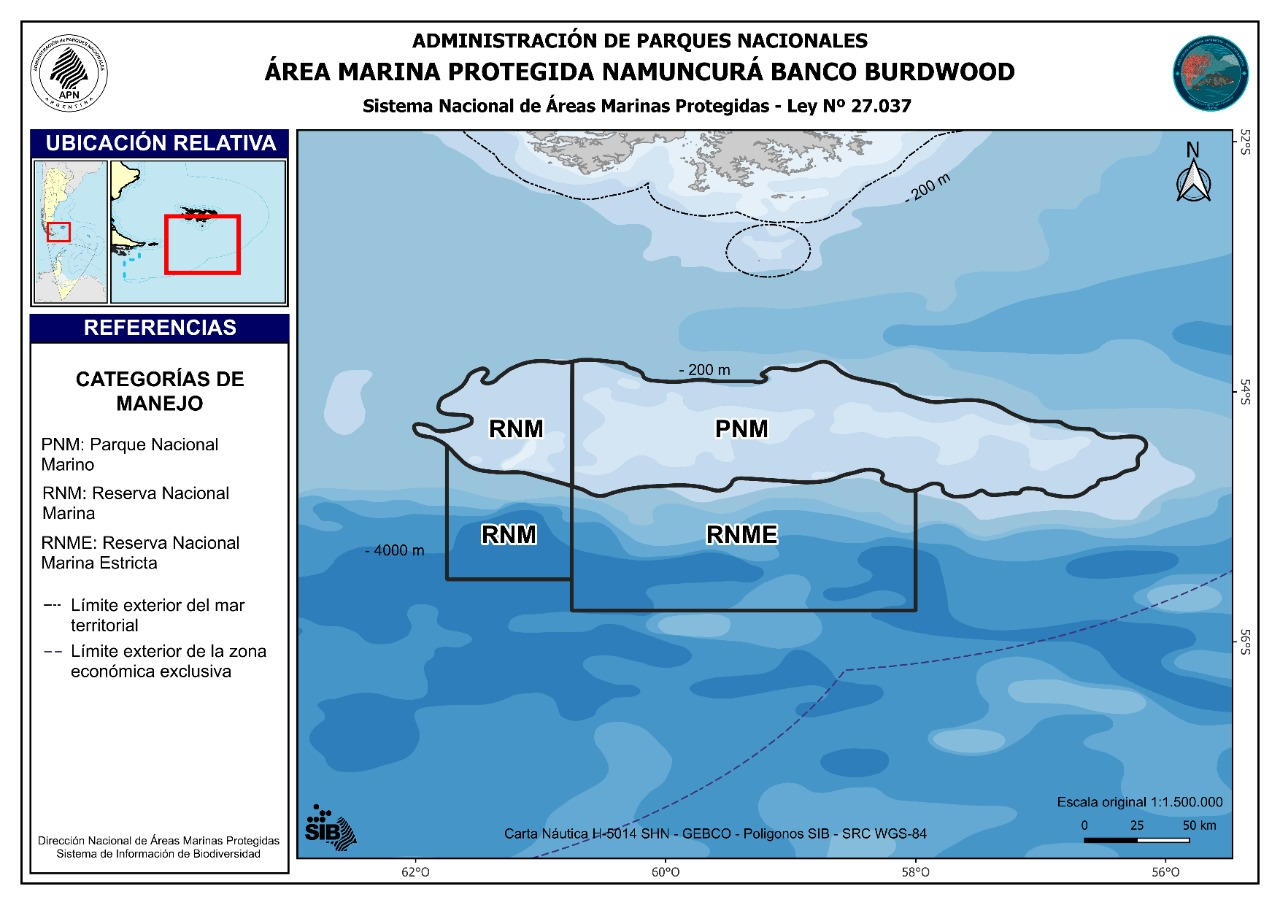
\includegraphics[width=1\linewidth]{MPABurdwood_map} \caption{Marine Protected Areas Namuncurá - Burdwood Bank I (MNR and MNP, northern section) and II (MNR and SMNR, southern section). Acronyms indicate categories according to the management plan: MNR - Marine National Reserve, MNP - Marine National Park and RMNR - Restricted Marine National Reserve.}\label{fig:figure1}
\end{figure}

\hypertarget{network-construction}{%
\subsection{Network construction}\label{network-construction}}

In order to build the network of predator-prey interactions, we reviewed
more than 170 references considering published articles, Ph.D.~theses,
public databases, and reports belonging to 16 research cruises conducted
in the MPAs N-BB I and II during 2014-2019. It is noteworthy that the
sampling effort was greater in the MPA N-BB I. Furthermore, we took into
account personal communications from experts belonging to the working
group of the study area
(https://www.pampazul.gob.ar/tag/banco-burdwood/). The diversity of the
authors' expertise contributing to the present study was a key factor in
enhancing the quality of the network, and inherently improved the
network representation. A list of the references used to build the
network is presented in Supplementary Material (Table S1).

Due to a lack of trophic data resolution for some species inhabiting the
study area, we followed the concept of trophic species, here defined as
follows: taxa collapsed into a single node in the network. In most
cases, we followed this concept when specific data on species, in the
taxonomic sense, were not available. In some cases, we collapsed species
when taxa shared the same set of predators and prey (trophic similarity,
Martinez (1991)), one of the aggregation methods that better preserve
food web functional properties (Gauzens et al., 2013). In addition, for
endemic species (e.g.~bryozoan \emph{Burdwoodipora paguricola}) and
other species with no trophic studies so far, we inferred their feeding
interactions applying a conservative approach that assumes that the set
of prey and predators are at some point preserved in time. In those
cases we gathered information from upper taxonomic levels (i.e.~Genus,
Family, Order, Class, Phylum) as a good proxy variable (Morales-Castilla
et al., 2015; Pomeranz et al., 2019). Details about this can be found in
Supplementary Material (Table S2). Furthermore, we considered non-living
food sources, such as detritus and necromass, as prey species in the
food web context.

With the gathered trophic data, we constructed a matrix of pairwise
interactions; a value of 1 or 0 was assigned to each element a\_ij of
the matrix depending on whether the j-species preyed or not on the
i-species. Then we transformed such a matrix into an oriented graph with
L trophic interactions between S nodes or species. The orientation or
direction of the graph follows the flow of energy and matter in the
network, from prey to predator.

\hypertarget{network-analysis}{%
\subsection{Network analysis}\label{network-analysis}}

We analysed the MPA N-BB network of trophic interactions, or food web,
at two levels: A) network, considering species and interactions of the
whole network; and B) species, considering interactions and species
related to a particular species (Table 1).

The network-level analysis aims to characterise the food web in terms of
complexity and structure. For this, we calculated several network
properties commonly used to describe empirical food webs (Pascual and
Dunne, 2005): (1) number of species S; (2) number of interactions or
links L; (3) link density L/S; (4) connectance L/S\^{}2; (5) omnivory
Omn; and (6) small-world pattern. In order to explore the small-world
phenomenon, we analysed the characteristic path length (CPL) and the
clustering coefficient (CC). The CPL is the average shortest path length
between all pairs of nodes (Watts and Strogatz, 1998). Here, CPL was
calculated as the average number of nodes in the shortest path
\(CPL_{Min} (i,j)\) between all pairs of nodes \(S(i,j)\) in a network
averaged over \(S(S-1)/2\) nodes:

\[
CPL = \frac{2}{S(S-1)} \sum_{i = 1}^{S} \sum_{i = 1}^{S} {CPL_{Min}(i,j)}
\] The CC quantifies the local interconnectedness of the network and it
is defined as the fraction of the number of existing links between
neighbours of node \(i\) among all possible links between these
neighbours. In this study, the CC was determined as the average of the
individual clustering coefficients \(CC_i\) of all the nodes in the
network. Individual \(CC_i\) were determined as follows:

\[
CC_i = \frac{2E_i}{K_i(K_i-1)}
\] where \(E_i\) is the effective number of interactions between \(K_i\)
nearest-neighbour nodes of node \(i\) and the maximal possible number of
such interactions (Newman, 2003). To test whether the food web presented
the small-world pattern, we compared the empirical values of CPL and CC
with those resulting from 1000 randomly generated networks with the same
size (S) and number of interactions (L), following the method proposed
by Marina et al. (2018b).

Also, we estimated the (7) degree distributions for the food web, prey
and predators, and each functional group (e.g., Amphipoda, Ascidiacea,
Bivalvia, fish, marine mammals, seabirds, among others). The prey and
predator distributions indicate the frequency of prey among predators,
and viceversa; the functional group's degree shows the distribution of
interactions within groups.

The species-level analysis aims to describe the species' role in the
food web. For this, we considered the following properties: betweenness
Btw, closeness Cl, trophic similarity TS, topological role TR, and
trophic level TL (Table 1). Topological roles refer to the fact that
food webs tend to naturally organize in non-random, modular patterns,
where modules are defined as a group of species that interact more
frequently among themselves than with species that are not members of
the module (Guimerà and Nunes Amaral, 2005). Species can play different
roles in this respect, according to the pattern of interactions within
their own module and/or across modules. We computed the topological role
for each species, classified as module hub, species with a relatively
high number of interactions, but most within its own module; module
specialist, species with relatively few interactions and most within its
own module; module connector, species with relatively few interactions
mainly between modules; and network connector, species with high
connectivity between and within modules (Guimerà and Nunes Amaral,
2005).

We also studied the relationship between species TL and the other
species properties by performing linear regression analyses. Thus, we
considered the TL as the dependent variable and the given property
(i.e.~betweenness, closeness, trophic similarity) as the independent
variable and obtained the coefficients (slope and intercept) for the
linear model. Models were fitted using the least squares approach. We
also explored the topological role categories with the species TL. These
species-level properties provide an appropriate description of species'
role in empirical complex food webs (Cirtwill et al., 2018).

All network analyses and graphs were performed in R version 4.2.2 (Team,
2022), mainly using `igraph' (Csardi and Nepusz, 2006) and `multiweb'
(Saravia, 2022) packages. The source code and data are available at
https://github.com/TomasMarina/Banco-Burdwood.

\begin{longtable}[]{@{}
  >{\raggedright\arraybackslash}p{(\columnwidth - 6\tabcolsep) * \real{0.2266}}
  >{\raggedright\arraybackslash}p{(\columnwidth - 6\tabcolsep) * \real{0.2578}}
  >{\raggedright\arraybackslash}p{(\columnwidth - 6\tabcolsep) * \real{0.2578}}
  >{\raggedleft\arraybackslash}p{(\columnwidth - 6\tabcolsep) * \real{0.2578}}@{}}
\caption{List of network and species-level properties analysed,
definitions, and relevant ecological implications related to food web
complexity and structure.}\tabularnewline
\toprule\noalign{}
\begin{minipage}[b]{\linewidth}\raggedright
\textbf{Name}
\end{minipage} & \begin{minipage}[b]{\linewidth}\raggedright
\textbf{Definition}
\end{minipage} & \begin{minipage}[b]{\linewidth}\raggedright
\textbf{Implications}
\end{minipage} & \begin{minipage}[b]{\linewidth}\raggedleft
\textbf{Reference}
\end{minipage} \\
\midrule\noalign{}
\endfirsthead
\toprule\noalign{}
\begin{minipage}[b]{\linewidth}\raggedright
\textbf{Name}
\end{minipage} & \begin{minipage}[b]{\linewidth}\raggedright
\textbf{Definition}
\end{minipage} & \begin{minipage}[b]{\linewidth}\raggedright
\textbf{Implications}
\end{minipage} & \begin{minipage}[b]{\linewidth}\raggedleft
\textbf{Reference}
\end{minipage} \\
\midrule\noalign{}
\endhead
\bottomrule\noalign{}
\endlastfoot
\textbf{Number of species} & Number of trophic species in a food web. &
It represents the species diversity and has implications for the
persistence of the ecosystem. & May 1973, Tilman 1996 \\
\textbf{Number of interactions} & Total number of trophic interactions
in a food web. & It represents the number of pathways along which matter
and energy can flow. & Dunne et al.~2002 \\
\textbf{Link density} & Ratio of interactions to species in a food web &
It represents the average number of interactions per species; informs
about how connected species are in the food-web. & Dunne et al.~2002 \\
\textbf{Connectance} & Proportion of potential links among species that
are actually realized. Range = 0 - 1. & It measures the probability of
interactions and is a fundamental measure of network complexity.
Connectance can be negatively or positively associated with food web
robustness, depending on the network structure (random vs non-random) or
how the strength of the interactions are distributed. & Martinez 1992 \\
\textbf{Degree distribution} & Frequency of trophic species that have k
or more interactions. & It suggests on the vulnerability of complex food
webs against random failures and intentional attacks (i.e. species
extinctions). & Albert \& Barabási 2002 \\
\textbf{Omnivory} & Species feeding on prey from more than one trophic
level. & It influences food web's stability; intermediate levels of
omnivory may stabilize it and may diffuse top-down effects thus reduce
the probability of trophic cascades. & McCann \& Hastings 1997 \\
\textbf{Small-world pattern} & A network with short path length
(distance between nodes) and high clustering coefficient (formation of
compartments) compared to random networks. & Consequences of this
structural pattern in food webs are of great importance in recognizing
evolutionary paths and the vulnerability to perturbations. & Watts \&
Strogatz 1998, Montoya \& Solé 2002 \\
\textbf{Betweenness} & Number of shortest paths going through a species.
& Species with high betweenness act as ``bridges''; if removed, would
have rapidly spreading effects in the food web. & Freeman 1978, Lai et
al.~2012 \\
\textbf{Closeness} & Number of steps required to reach every other
species from a given species. & The removal of a species with high
closeness will affect the most other species in the food web. & Freeman
1978, Lai et al.~2012 \\
\textbf{Trophic similarity} & Trophic overlap based on shared and unique
resources (prey) and consumers (predators). & It measures one of the
most important aspects of species' niches, the trophic niche, and
functional aspects of biodiversity. & Martinez 1992 \\
\textbf{Topological role} & Species role according to interactions
within and across modules (subgroups of species). & Four roles are
defined: module hub, module specialist, module connector and network
connector. Network connector and module connector roles maintain the
connectivity of the food web. & Guimera \& Nunes Amaral 2005 \\
\end{longtable}

\hypertarget{results}{%
\section{Results}\label{results}}

\hypertarget{network-level-properties}{%
\subsection{Network-level properties}\label{network-level-properties}}

In terms of complexity, the MPA Namuncurá - Burdwood Bank food web
consisted of 1788 predator-prey interactions and 379 species, where 93\%
of them were defined at the species taxonomical level (Figure 2, Table
S2). The food web presented a link density (e.g., the average number of
interactions per species) of 4.72, and a connectance of 0.01. Almost
half of the consumers were omnivores (0.48), feeding on sources at
different trophic levels. The food web displayed a small-world pattern,
meaning that the path length was lower and the clustering coefficient
higher than the random networks (Table 2).

\newpage

\begin{figure}

{\centering 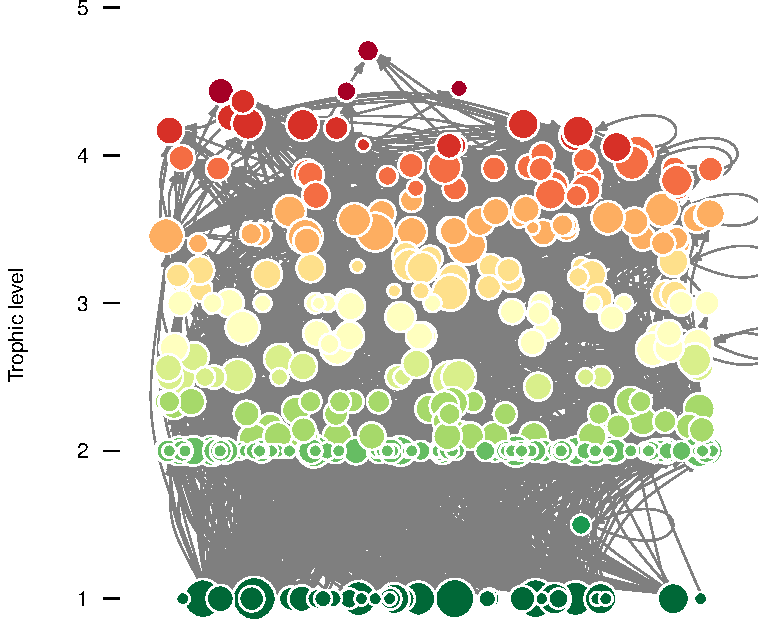
\includegraphics{MS_Burdwood_foodweb_files/figure-latex/figure2-1} 

}

\caption{Graph of the food web for the MPA Namuncurá - Burdwood Bank. Circles represent species and arrows trophic interactions. Circle diameter is relative to the number of interactions. Colour gradient indicates the trophic level.}\label{fig:figure2}
\end{figure}

\begin{table}

\caption{\label{tab:table2}Network-level properties of the MPA Namuncurá - Burdwood Bank food web. CPL: Characteristic Path Length; CC: Clustering Coefficient; SW: Small-World pattern. See table 1 for definitions and ecological relevance.}
\centering
\begin{tabular}[t]{r|r|r|r|r|r|r|l}
\hline
\textbf{Species} & \textbf{Interactions} & \textbf{Density} & \textbf{Connectance} & \textbf{Omnivory} & \textbf{CPL} & \textbf{CC} & \textbf{SW}\\
\hline
379 & 1788 & 4.72 & 0.01 & 0.49 & 2.99 & 0.08 & True\\
\hline
\end{tabular}
\end{table}

The degree distribution of the food web showed an asymmetric frequency
in the number of interactions, where most of the species had a
relatively low number of interactions and few species concentrated most
of them (Figure 3A). The distribution of prey among predators showed
that most consumers fed on a low number of prey whereas few had multiple
prey (Figure 3B). The top-five predators in number of prey were:
yellowfin notothen \emph{Patagonotothen guntheri} (Notothenioid fish, 50
prey), rock cod \emph{Patagonotothen ramsayi} (Notothenioid fish, 49
prey), broad nose skate \emph{Bathyraja brachyurops} (Chondrichthyan, 33
prey), Patagonian toothfish \emph{Dissostichus eleginoides}
(Notothenioid fish, 30 prey), and graytail skate \emph{Bathyraja
griseocauda} (Chondrichthyan, 28 prey). Following the same distribution
pattern, few prey presented multiple predators (Figure 3C). The top-five
prey (or food sources) in number of predators were: Detritus
(Non-living, 153 predators), the three categories of Diatoms considered
(benthic, centric and pennate, 72.5 predators on average), and species
of the genus \emph{Euphausia} (Zooplankton, 46 predators). Finally,
taking into account the interactions within each functional group, most
interactions were concentrated in a few species (Figure 3D). The most
evident species were: \emph{Doryteuthis gahi} (Cephalopoda),
\emph{Grimothea (=Munida) gregaria} (Decapoda), \emph{Patagonotothen
ramsayi}, \emph{Patagonotothen guntheri} and \emph{Dissostichus
eleginoides} (bentho-pelagic fish), \emph{Sprattus fuegensis} and
\emph{Micromesistius australis} (pelagic fish), and species of
\emph{Euphausia} and \emph{Themisto gaudichaudii} (Zooplankton).
Overall, there is an evident asymmetry in the distribution of
interactions among species at different levels in the MPA N-BB food web.

A list of the distribution of interactions per species is presented in
Supplementary Material (Table S3).

\begin{figure}

{\centering 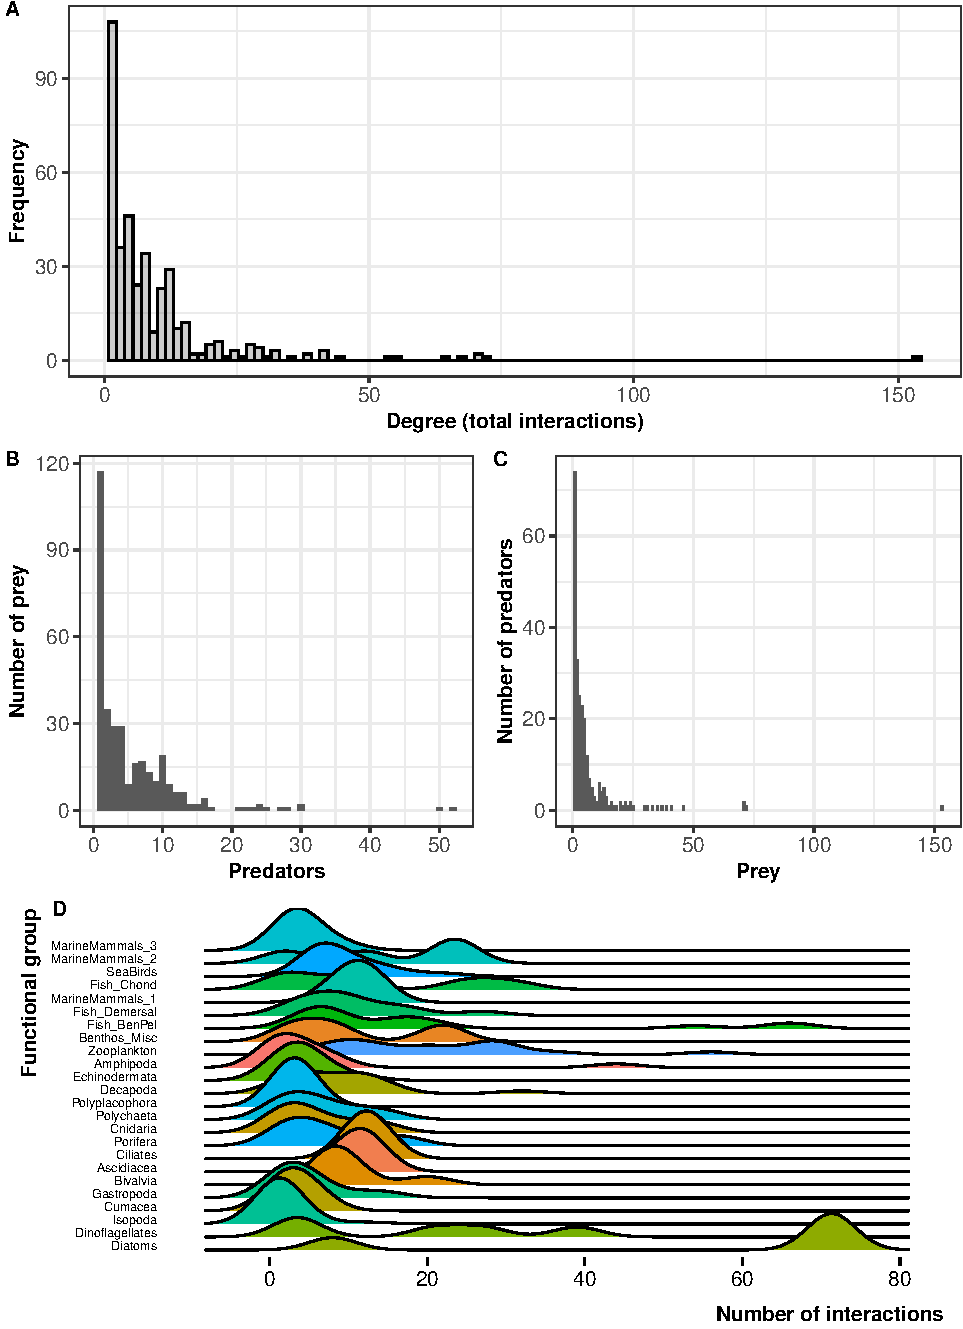
\includegraphics{MS_Burdwood_foodweb_files/figure-latex/figure3-1} 

}

\caption{Degree distributions for the (A) food web, for (B) prey among predators, (C) predators among prey, and (D) for each functional group. Groups are vertically ordered by increasing trophic level (following coloration of figure 2); groups with less than 3 species were not plotted (e.g., pelagic fish). All functional groups and the species that comprise them are shown in Supplementary Material (Table S3).}\label{fig:figure3}
\end{figure}

\hypertarget{species-level-properties}{%
\subsection{Species-level properties}\label{species-level-properties}}

We found different relationships between the species trophic level (TL)
and the rest of the analysed species-level properties (Figure 4A-D). The
most evident significant relationship was with trophic similarity,
i.e.~the higher the species' TL, the lower the trophic similarity or the
higher the uniqueness in terms of trophic role (Figure 4C). Here it is
noteworthy to highlight those high-trophic level species (TL
\textgreater{} 3.1) with low values of trophic similarity:
\emph{Bathyraja macloviana} and \emph{Squalus acanthias}
(Chondrichthyans), \emph{Diplopteraster clarki} and \emph{Pteraster} sp.
(echinoderms), \emph{Daption capense} and \emph{Eudyptes chrysocome}
(seabirds), Ziphiidae and \emph{Lagenorhynchus cruciger} (marine
mammals) (Table S3).

We also found a significant negative relationship between TL and
closeness, however less evident, meaning that low-TL species are
relatively closer to any other species in the food web (Figure 4B).
Detritus, species of genera \emph{Calanus} and \emph{Euphausia}, and
Foraminifera, all with TL \textless{} 3, registered the highest
closeness values (Table S3).

Notably, species of mid-TLs (3-4.2) showed the highest values of
betweenness, meaning that those species participated in the highest
number of shortest paths between species (Figure 4A). The following are
the species with the highest values (descending order):
\emph{Patagonotothen ramsayi}, \emph{Salilota australis},
\emph{Dissostichus eleginoides} (fishes), \emph{Doryteuthis gahi}
(Cephalopoda), and \emph{Patagonotothen guntheri} (Notothenioid fish)
(Table S3).

Considering the topological role, `module specialist' species were the
most frequent and presented a wide TL range (1 - 4.78), as well as
`module hub' species (TL = 1 - 3.92); `module connector' was constrained
to mid-TLs (2 - 3.86); and `network connector', was represented by only
one trophic species: detritus (Figure 4D, see Figure S2 for species'
topological roles in a food web graph framework). Here it is important
to highlight the two latter topological roles because they are
responsible for linking modules and maintaining the connectivity of the
food web: 42 species (1 network connector + 41 module connectors) from
19 different functional groups with a TL range = 1 - 3.86. The 41
species with a module connector role represented these functional
groups: Amphipoda, Bivalvia, Brachiopoda, Bryozoa, Hydrozoa (as
`Cnidaria\_benthic'), Copepoda, Cumacea, Decapoda, Echinodermata, fish
(bentho-pelagic and demersal Osteichthyes, and Chondrychthyes),
Foraminifera, Polychaeta, Porifera, Pycnogonida (as `Benthos\_Misc') and
zooplankton (see Supplementary Material Table S3 for the identity of the
species).

An exhaustive list of the species-level properties is presented in
Supplementary Material (Table S3).

\begin{figure}

{\centering 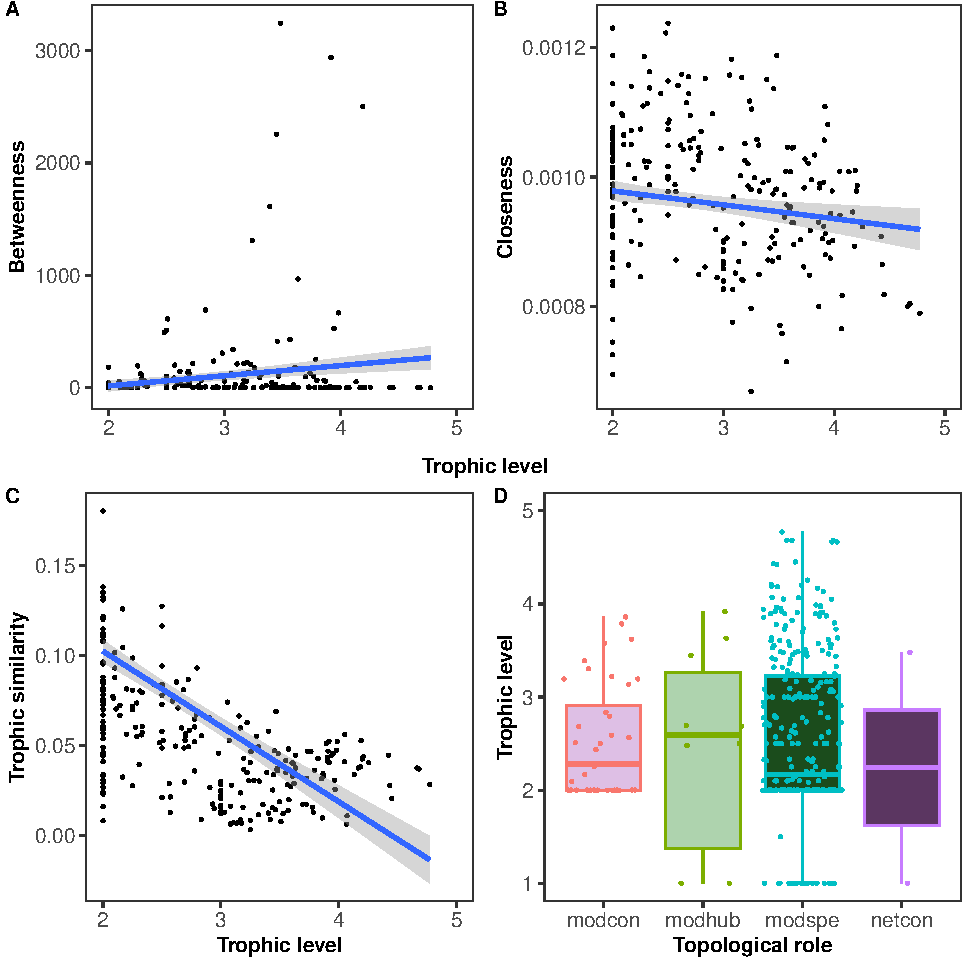
\includegraphics{MS_Burdwood_foodweb_files/figure-latex/figure4-1} 

}

\caption{Species-level properties by trophic level: (A) betweenness, (B) closeness, (C) trophic similarity, and (D) topological role. Each point represents a species. Linear regressions for betweenness ($y = 74.97x - 117.35, R^2 = 0.05, p-value < 0.01$), closeness ($y = 9.33e-06x - 9.31e-4, R^2 = 0.003, p-value = 0.15$) and trophic similarity ($y = -0.02x + 0.11 , R^2 = 0.07, p-value < 0.01$). Note that for panels A, B and C only species with TLs equal or greater than 2 were considered.}\label{fig:figure4}
\end{figure}

\hypertarget{discussion}{%
\section{Discussion}\label{discussion}}

\hypertarget{the-food-web-of-the-mpa-namuncuruxe1---burdwood-bank-ecosystem}{%
\subsection{The food web of the MPA Namuncurá - Burdwood Bank
ecosystem}\label{the-food-web-of-the-mpa-namuncuruxe1---burdwood-bank-ecosystem}}

The food web of the MPA N-BB ecosystem analysed in this study is one of
the most highly-resolved networks of trophic interactions ever studied,
not only for a high-latitude open-ocean ecosystem but also for any
marine protected area worldwide to our knowledge. It is of paramount
importance to consider the complexity of species interactions in order
to gain insights into the structure and functioning of the ecosystem,
since the aggregation of species might mask food web properties and
produce type II errors (false positives) (Gauzens et al., 2013;
Martinez, 1993).

Food web connectance is a feature that resumes the complexity of the
network, but more importantly, it is an emergent property of pairwise
species interactions (Poisot and Gravel, 2014). It contains information
regarding how interactions within an ecological network are distributed
and predicts reasonably well key dynamical properties of ecological
networks (Jennifer A. Dunne et al., 2002a). Complex marine food webs
(i.e.~with more than 25 trophic species) show connectance values ranging
from 0.01 - 0.27 (Marina et al., 2018b). In particular, food webs from
high-latitude regions tend to exhibit a connectance closer to the
minimum (between 0.01 and 0.05) (Kortsch et al., 2015; Rodriguez et al.,
2022; Santana et al., 2013). Whether food webs display a low or a high
connectance helps to better comprehend ecosystem's synthetic properties
like robustness. In this sense, empirical analyses support the notion
that highly-connected ecological networks are robust against external
perturbations such as the introduction of new (e.g., invasive) species
(Smith-Ramesh et al., 2017) as well as species removal (e.g., local
extinction) (Jennifer A. Dunne et al., 2002b; Montoya and Solé, 2003).
The connectance of the food web of the MPA Namuncurá - Burdwood Bank
(0.01) is one of the lowest reported so far for these regions; in
particular, it appears to be much lower than that of Beagle Channel
(0.05), an adjacent coastal area (Rodriguez et al., 2022).

The degree distribution, the distribution of the number of interactions
per species, is the core of the structure of species interactions, which
influences the opportunities for multiple species to persist in the long
term and, therefore, their coexistence (Godoy et al., 2018). The food
web for the MPA N-BB presents an asymmetric degree distribution. This
pattern was identified at different levels of analysis: food web,
predator, prey, and functional group. Such asymmetry is a well-known
feature in empirical complex food webs in particular (Jennifer A. Dunne
et al., 2002a; Montoya and Solé, 2003; Stouffer et al., 2005), and has
received great attention in complex networks in general (Albert and
Barabási, 2002; Newman, 2003). The degree distribution affects the
resilience of complex food webs against random failures and pressure on
a particular component of the web: food webs showing right-skewed
distributions, like the one described in this study, are more vulnerable
to the removal of the most connected species or hubs, with the potential
of producing secondary extinctions and a catastrophic fragmentation of
the network (Albert et al., 2000; Jennifer A. Dunne et al., 2002b; Eklöf
and Ebenman, 2006).

It is suggested that the small-world pattern, i.e., a network with short
path length and high clustering coefficient, is not frequent in complex
marine food webs, mainly due to a low clustering coefficient compared to
random networks (Jennifer A. Dunne et al., 2002c; Marina et al., 2018b).
However, the food web of the MPA N-BB does display a small-world
pattern. Consequences of this could be of great importance in
recognizing species evolutionary paths and the vulnerability to
perturbations (Montoya and Solé, 2002). On the one hand, a short path
length implies a rapid spread of an impact (e.g., contaminant,
population fluctuation, local extinction) throughout the network but, at
the same time, more potentially adaptive dynamics in the face of
external perturbations (Montoya and Solé, 2002; Williams et al., 2002).
On the other hand, a high clustering coefficient indicates the formation
of subnetworks composed only by the neighbours of particular species.
This translates into a greater resistance of the network due to the
confinement of perturbations mainly within subnetworks and not spreading
between them (Heer et al., 2020; Kortsch et al., 2019). Overall, a
small-world topology provides ecological networks with greater
resilience and resistance (Bornatowski et al., 2017; Dormann et al.,
2017).

Omnivory acts as a buffer to changes as the ecosystem presents
alternative energy pathways in the face of perturbations, i.e., reducing
the risk of cascading extinctions following the primary loss of species
(Borrvall et al., 2000). Omnivores are species able to adapt faster and
to a broader range of environmental conditions by changing their
foraging habits to feed on the most abundant prey (Fagan, 1997).
Furthermore, omnivory can be analysed from the interaction point of
view: theoretical studies have identified omnivorous interactions as a
possible candidate for a keystone interaction, sensu Kadoya et al.
(2018), highlighting the importance of omnivory in stabilizing food web
dynamics (McCann and Hastings, 1997; Neutel et al., 2002). The high
proportion of omnivory in the food web of the MPA N-BB suggests that the
network might be robust to variations in prey abundances, which could
increase food web's persistence and stability (Stouffer and Bascompte,
2010).

In summary, the food web of the MPA N-BB presents a combination of
network properties that makes it unique in terms of network resolution,
complexity, and structural pattern. All this suggests that the food web
might be fragile to external perturbations targeting highly connected
species, which in turn coincides to be commercial exploited species as
fishes (Laptikhovsky et al., 2013; Martínez et al., 2015; Winter and
Arkhipkin, 2023). However, structural properties might provide
resilience and resistance with the final outcome of a rearranged
structure maintaining its functions.

\hypertarget{dominant-consumers-and-food-sources}{%
\subsection{Dominant consumers and food
sources}\label{dominant-consumers-and-food-sources}}

The degree distribution allows identifying important species, such as
potential keystone species (i.e.~highly connected) (Jennifer A. Dunne et
al., 2002b; Solé and Montoya, 2001), generalist/specialist species, and
dominant food sources (Kondoh et al., 2010).

We have identified that most of the consumers in the food web of the MPA
N-BB either have a narrow diet or are specialists, while few present a
broad or generalist diet. The most evident generalist species are
\emph{Patagonotothen guntheri} (Covatti Ale et al., 2022), \emph{P.
ramsayi} (Fischer et al., 2022), juveniles of \emph{Dissostichus
eleginoides} (Troccoli et al., 2020), \emph{Bathyraja brachyurops}
(Belleggia et al., 2008), and \emph{B. griseocauda} (Bellegia et al.,
2014), with more than 25 potential prey. Since these species present
mid-trophic positions in the food web (with the exception of adults of
\emph{Dissostichus eleginoides} that are top predators), acting as
predator and prey, they might be important links between lower and
higher trophic levels. This result is in agreement with the sole
analysis, using stable isotopes, that exists so far for the trophic
structure of the MPA N-BB (Riccialdelli et al., 2020), and resembles
other high-latitude marine systems of the Southwest Atlantic and
Antarctic regions (Arkhipkin and Laptikhovsky, 2013; Marina et al.,
2018a). The importance of these particular generalist species also
arises since they feed in the benthic and pelagic habitats (Covatti Ale
et al., 2022; Fischer et al., 2022; Troccoli et al., 2020), linking
these realms and contributing to the vertical carbon flow.

On the other hand, a low number of prey are consumed by many predators
in the food web of the MPA N-BB. This suggests that there are dominant
food sources on which most consumers depend and from where the ecosystem
energy is being transferred to the upper trophic levels. The most
demanded source we identified in this study (i.e.~detritus) supports the
abundant benthic community of filter-feeders (Schejter et al., 2016),
components of the animal forest (Schejter et al., 2020), likely feeding
on detritus that is constantly resuspended from the bottom (Martin and
Flores Melo, 2021). Furthermore, we found that the second and third-most
consumed prey were diatoms and species of \emph{Euphausia},
respectively, which are essential sources for the diverse zooplankton
community (Spinelli et al., 2020), mid-TL consumers like the Fuegian
sprat \emph{Sprattus fuegensis} (Padovani et al., 2021) and
\emph{Patagonotothen ramsayi} (Fischer et al., 2022), and top predators
such as the black-browed and grey-headed albatrosses (\emph{Thalassarche
melanophris} and \emph{Thalassarche chrysostoma}, respectively) (Catry
et al., 2004), and baleen whales (species of the genera
\emph{Balaenoptera} and \emph{Eubalaena}) (Valenzuela et al., 2018).

\hypertarget{species-role-related-to-their-trophic-level}{%
\subsection{Species' role related to their trophic
level}\label{species-role-related-to-their-trophic-level}}

Describing species' roles in food webs provides a toolbox to assess the
significance of species in terms of community's functioning and overall
stability (Cirtwill et al., 2018; Thébault and Fontaine, 2010). We used
a range of descriptors to characterise the dynamic and multifaceted
nature of the species forming the MPA N-BB food web.

Closeness and betweenness are defined as ``mesoscale'' properties
because they consider direct and indirect interactions, therefore
describing the focal species' ability to influence the rest of the
species of the food web (Lai et al., 2012). Closeness quantifies how
many steps away species \(i\) is from all other species in the food web,
and is proportional to how rapidly the indirect effects of the focal
species can spread to other species in the network (Scotti and Jordán,
2010). In the food web of the MPA N-BB, low-TL consumers arise as
important in this regard: species of the zooplankton community,
\emph{Calanus} and \emph{Euphausia}, \emph{Zygochlamys patagonica}
(Bivalvia), and Brachiopoda. Any perturbation affecting these species,
such as the recently confirmed contaminants mercury (Fioramonti et al.,
2022) and microplastics (Cossi et al., 2021; Di Mauro et al., 2022),
should be of concern since it might reach many other species in the food
web. Otherwise, betweenness measures the number of shortest paths
between species, providing information on the importance of species as
``bridges'' for energy transfer: a species with high betweenness takes
part in more food chains and therefore affects more energy flows (Scotti
and Jordán, 2010). We have identified the longtail southern cod
\emph{Patagonotothen ramsayi} as the most important species in this
sense. Moreover, in light of our analysis, other species like the
Patagonian toothfish \emph{Dissostichus eleginoides} (juveniles), the
Patagonian cod \emph{Salilota australis}, the yellowfin notothenioid
\emph{Patagonotothen guntheri}, and the Patagonian longfin squid
\emph{Doryteuthis gahi} should be considered as relevant in the energy
transfer in the ecosystem. All these species have a mid-trophic position
in the food web, supporting the `wasp-waist' control hypothesis for the
MPA N-BB (Riccialdelli et al., 2020).

Ecosystems with a pronounced `wasp-waist' structure are suggested to
present a high trophic redundancy, since many species would show similar
trophic habits (Cury et al., 2000). The significant negative
relationship between trophic similarity and trophic level enhances the
hypothesis of functional similarity at low and mid-TL species compared
to higher TL species for the MPA N-BB food web (Riccialdelli et al.,
2020). At the same time, our results highlight the uniqueness in terms
of the trophic role of high-TL predators. Here, not only the expected
pelagic animals such as marine mammals and seabirds arise as relevant,
but also demersal vertebrate (chondrichthyans \emph{Bathyraja
macloviana} and \emph{Squalus acanthias}) and benthic invertebrate
species (echinoderms \emph{Diplopteraster clarki} and \emph{Pteraster}
sp.) are noteworthy. The role that such species play in the MPA N-BB
ecosystem is unique and perturbations on them might result in
unprecedented changes at the trophic structure and functioning level. In
this regard, we should mention the potential threat of the fisheries
operating in the western section of the MPA N-BB, where this activity is
allowed and mostly focuses on the Patagonian toothfish
\emph{Dissostichus eleginoides} and the southern blue whiting
\emph{Micromesistius australis} (Martínez et al., 2015). Although the
fishing effort is concentrated outside the limits of the MPA N-BB, the
impact on the MPA ecosystem should not be neglected (Martínez et al.,
2021).

Species' role can also be assessed in a module-based context. Among the
varying numbers of topological roles in which species can be divided,
two are remarkable: `module connector' and `network connector'. Here,
our results point out that there are several species, belonging to a
wide range of trophic positions (1 to 3.86) and representing 17
different functional groups, that should be considered as influential
species for the connectivity of the food web. Thus, we propose that the
diversity of species (benthic and pelagic) maintains the connectivity of
the food web, therefore contributing to the trophic structure and
ecosystem's stability.

\hypertarget{caveats-and-future-perspectives}{%
\subsection{Caveats and future
perspectives}\label{caveats-and-future-perspectives}}

The food web studied in the present work might be more representative of
the shallow ecosystem of the submarine plateau called Burdwood Bank, on
which most of the research was focused as the MPA N-BB I was first
created. This is related to the sampling effort that was conducted
during the research cruises in the former MPA compared to the MPA N-BB
II (i.e.~deep flanks to the south). As a consequence, most of the data
we used to build the network come from studies performed in the MPA N-BB
I. Despite this fact, we decided to build the food web considering both
MPAs due to the tight oceanographic and ecological connection that
exists among them (Administración de Parques Nacionales, 2022 and
references therein).

It's important to mark that we did not consider quantitative data
(i.e.~abundance, biomass) to assess the species' role in the food web.
Although there exists such data for some species (Schejter and Albano,
2021), it would not be possible to include it in the food web framework
described here due to a taxonomical resolution mismatch. In this regard,
we should mention the case of \emph{Zygochlamys patagonica} (Bivalvia)
and Brachiopoda that are highlighted by our species-level analyses
though they have been found in low abundances in the area (Schejter and
Albano, 2021).

Some species of sessile suspension feeders in high-latitude marine
ecosystems, such as sponges, ascidians and octocorals, avoid predation
by producing secondary metabolites that function as a chemical defense
(Moles et al., 2015; Núñez-Pons et al., 2010; Prieto et al., 2022).
Although this was not yet recorded at the MPA N-BB, there are a few
studies that reported it in other locations in species that inhabit the
MPA N-BB (Rojo de Almeida et al., 2010).

The MPA N-BB I presents complex oceanographic conditions that generate
an internal spatial heterogeneity, mainly along its longitudinal axis
(Matano et al., 2019). So far this heterogeneity has been reflected in
phytoplankton and zooplankton communities (Bértola et al., 2018; García
Alonso et al., 2020; Spinelli et al., 2020), and in fish assemblages
(Delpiani et al., 2020). Moreover, seasonal variations also occur in
some physical and biological aspects of the MPA N-BB I (García Alonso et
al., 2018; Matano et al., 2019). Considering both MPAs (N-BB I and II),
a seasonal variation in the community composition of marine mammals and
seabirds was recorded recently (Dellabianca et al., 2023). The spatial
and seasonal variations in the plankton community might affect the
energy and matter flow to higher levels of the food web. This has been
recently studied in the vicinity of the MPA N-BB I, in the Beagle
Channel, where a differential energy flow pattern of the plankton
community has been recognised in two micro-basins of the Channel
separated by a sill, each with different physicochemical properties
(Giesecke et al., 2021), nutrient concentration (Latorre et al., 2023)
as well as in the dominant component of the plankton community (Bruno et
al., 2023; Presta et al., 2023). Although we were aware of the above, we
decided to characterise a food web representing the whole MPA N-BB I
year round since this is the first study of its type in the area.

Taking into account the mentioned caveats, and with the aim of improving
the knowledge regarding the structure, functioning and stability of the
MPA N-BB, we suggest that the future perspectives should: 1) incorporate
spatial heterogeneity among MPA N-BB I and II (Schejter and Albano,
2021), which might lead to distinct food web properties in terms of
structure and functioning (Cordone et al., 2020; Kortsch et al., 2019);
2) include species traits, like body size and mass, since they are known
to be important drivers in predator-prey interactions (Brose et al.,
2019); 3) simulate the anthropogenic impacts already present in the MPA
N-BB ecosystem (e.g.~microplastics, mercury) (Cossi et al., 2021; Di
Mauro et al., 2022; Fioramonti et al., 2022) as perturbations within the
framework of the described complex food web; and 4) estimate the
interaction strength of each predator-prey relationship in the food web
considering species and interaction traits (i.e.~body size, body mass,
interaction dimensionality), and species density data (Nilsson and
McCann, 2016; Pawar et al., 2012).

\hypertarget{conclusion}{%
\section{Conclusion}\label{conclusion}}

We compiled information on the species and trophic diversity of the
oceanic Marine Protected Area Namuncurá - Burdwood Bank, generating an
unprecedented, well-resolved network of trophic interactions for a
sub-Antarctic ecosystem, identifying the complexity and structure of the
system, and the main species role in a network framework. Particular
properties at the network level allowed us to identify the ecosystem's
vulnerability and potential response to perturbations in the presence of
highly-connected species, with a rearranged structure maintaining their
functions due to its potential resilience and resistance.

We identified several species as important regarding different aspects
of trophic structure and functioning, and response to perturbations
(i.e.~environmental/anthropogenic changes). On the one hand, we suggest
that generalist species, mainly fishes, play a crucial role in the
ecosystem's bentho-pelagic coupling process. At the same time, we
propose that other species besides the longtail southern cod
\emph{Patagonotothen ramsayi} and the Fueguian sprat \emph{Sprattus
fuegensis} should be considered relevant energy transfers for the
ecosystem. Finally, we argue that it is the diversity of species,
representing the benthic and pelagic habitats, that maintains the
connectivity of the food web against perturbations, therefore
contributing to the structure and stability of the ecosystem.

\hypertarget{acknowledgements}{%
\section{Acknowledgements}\label{acknowledgements}}

We are indebted to all those experts of the working group `Banco
Burdwood' who humbly provided their knowledge to enhance the quality of
the present research. Although most of them are authors of the present
work, it is worth to mention the following researchers: Brenda L. Doti
(IBBEA, CONICET-UBA; Universidad de Buenos Aires, Argentina), Sofía L.
Callá (Museo Argentino de Ciencias Naturales ``Bernardino Rivadavia'',
Argentina), Sandra Gordillo (IDACOR-CONICET; Universidad Nacional de
Córdoba, Argentina), Mariano I. Martinez (Museo Argentino de Ciencias
Naturales ``Bernardino Rivadavia'', Argentina) and Luciano Padovani
(Instituto Nacional de Investigación y Desarrollo Pesquero, INIDEP,
Argentina). We thank the MPA Namuncurá − Burdwood Bank administration.
Research cruises were funded by national funds by the Law 26.875. This
study was funded by Consejo Nacional de Investigaciones Científicas y
Técnicas (CONICET) and Agencia Nacional de Promoción Científica y
Tecnológica (PICT 2020-SERIEA-01617), Argentina. This work is
contribution no. XX of the MPA Namuncurá (Law 26.875).

\hypertarget{literature-cited}{%
\section*{Literature Cited}\label{literature-cited}}
\addcontentsline{toc}{section}{Literature Cited}

\hypertarget{refs}{}
\begin{CSLReferences}{1}{0}
\leavevmode\vadjust pre{\hypertarget{ref-Acha2004}{}}%
Acha, E.M., Mianzan, H.W., Guerrero, R.A., Favero, M., Bava, J., 2004.
\href{https://doi.org/10.1016/j.jmarsys.2003.09.005}{Marine fronts at
the continental shelves of austral {South America}: {Physical} and
ecological processes}. Journal of Marine Systems 44, 83--105.

\leavevmode\vadjust pre{\hypertarget{ref-AdministraciondeParquesNacionales2022}{}}%
Administración de Parques Nacionales, 2022. {Plan de gestión AMP
Namuncurá Banco Burdwood}.

\leavevmode\vadjust pre{\hypertarget{ref-Albert2002}{}}%
Albert, R., Barabási, A.-L., 2002.
\href{https://doi.org/10.1103/RevModPhys.74.47}{Statistical mechanics of
complex networks}. Reviews of Modern Physics 74, 47--97.

\leavevmode\vadjust pre{\hypertarget{ref-Albert2000}{}}%
Albert, R., Jeong, H., Barabási, A.-L., 2000.
\href{https://doi.org/10.1038/35019019}{Error and attack tolerance of
complex networks}. Nature 406, 378--382.

\leavevmode\vadjust pre{\hypertarget{ref-Arkhipkin2013}{}}%
Arkhipkin, A., Laptikhovsky, V., 2013.
\href{https://doi.org/10.1111/jfb.12217}{From gelatinous to muscle food
chain: Rock cod {Patagonotothen} ramsayi recycles coelenterate and
tunicate resources on the {Patagonian Shelf}}. Journal of Fish Biology
83, 1210--1220.

\leavevmode\vadjust pre{\hypertarget{ref-Bascompte2009}{}}%
Bascompte, J., 2009.
\href{https://doi.org/10.1126/science.1170749}{Disentangling the {Web}
of {Life}}. Science 325, 416--419.

\leavevmode\vadjust pre{\hypertarget{ref-Belleggia2008a}{}}%
Belleggia, M., Mabragaña, E., Figueroa, D.E., Scenna, L.B., Barbini,
S.A., Astarloa, J.M.D. de, 2008.
\href{https://doi.org/10.3989/scimar.2008.72n4701}{Food habits of the
broad nose skate, {\emph{Bathyraja}}{ \emph{Brachyurops}}
({Chondrichthyes}, {Rajidae}), in the south-west {Atlantic}}. Scientia
Marina 72, 701--710.

\leavevmode\vadjust pre{\hypertarget{ref-Bellegia2014}{}}%
Bellegia, M., Scenna, L., Barbini, S.A., Figueroa, D.E., Díaz de
Astarloa, J.M., 2014.
\href{https://doi.org/10.26028/CYBIUM/2014-384-012}{The diets of four
{Bathyraja} skates ({Elasmobranchii}, {Arhynchobatidae}) from the
{Southwest Atlantic}}.

\leavevmode\vadjust pre{\hypertarget{ref-Bertola2018}{}}%
Bértola, G., Olguín Salinas, H., Alder, V.A., 2018. Distribución
espacial de {Rhizosolenia} crassa, \textquestiondown especie clave del
banco burdwood? In: Libro de Resúmenes {X Jornadas Nacionales} de
{Ciencias} Del {Mar}. {Ciudad Autónoma de Buenos Aires, Argentina}.

\leavevmode\vadjust pre{\hypertarget{ref-Bornatowski2017}{}}%
Bornatowski, H., Barreto, R., Navia, A.F., de Amorim, A.F., 2017.
\href{https://doi.org/10.1111/maec.12407}{Topological redundancy and
{``small-world''} patterns in a food web in a subtropical ecosystem of
{Brazil}}. Marine Ecology 38, e12407.

\leavevmode\vadjust pre{\hypertarget{ref-Borrvall2000}{}}%
Borrvall, C., Ebenman, B., Tomas Jonsson, T.J., 2000.
\href{https://doi.org/10.1046/j.1461-0248.2000.00130.x}{Biodiversity
lessens the risk of cascading extinction in model food webs}. Ecology
Letters 3, 131--136.

\leavevmode\vadjust pre{\hypertarget{ref-Brose2019}{}}%
Brose, U., Archambault, P., Barnes, A.D., Bersier, L.-F., Boy, T.,
Canning-Clode, J., Conti, E., Dias, M., Digel, C., Dissanayake, A.,
Flores, A.A.V., Fussmann, K., Gauzens, B., Gray, C., Häussler, J., Hirt,
M.R., Jacob, U., Jochum, M., Kéfi, S., McLaughlin, O., MacPherson, M.M.,
Latz, E., Layer-Dobra, K., Legagneux, P., Li, Y., Madeira, C., Martinez,
N.D., Mendonça, V., Mulder, C., Navarrete, S.A., O'Gorman, E.J., Ott,
D., Paula, J., Perkins, D., Piechnik, D., Pokrovsky, I., Raffaelli, D.,
Rall, B.C., Rosenbaum, B., Ryser, R., Silva, A., Sohlström, E.H.,
Sokolova, N., Thompson, M.S.A., Thompson, R.M., Vermandele, F., Vinagre,
C., Wang, S., Wefer, J.M., Williams, R.J., Wieters, E., Woodward, G.,
Iles, A.C., 2019.
\href{https://doi.org/10.1038/s41559-019-0899-x}{Predator traits
determine food-web architecture across ecosystems}. Nature Ecology \&
Evolution 3, 919--927.

\leavevmode\vadjust pre{\hypertarget{ref-Bruno2023a}{}}%
Bruno, D.O., Valencia-Carrasco, C., Paci, M.A., Leonarduzzi, E., Castro,
L., Riccialdelli, L., Iachetti, C.M., Cadaillon, A., Giesecke, R.,
Schloss, I.R., Berghoff, C.F., Martín, J., Diez, M., Cabreira, A.,
Presta, M.L., Capitanio, F.L., Boy, C.C., 2023.
\href{https://doi.org/10.1016/j.jmarsys.2023.103876}{Spring plankton
energy content by size classes in two contrasting environments of a high
latitude ecosystem: {The Beagle Channel}}. Journal of Marine Systems
240, 103876.

\leavevmode\vadjust pre{\hypertarget{ref-Catry2004}{}}%
Catry, P., Phillips, R.A., Phalan, B., Silk, J.R.D., Croxall, J.P.,
2004. \href{https://doi.org/10.3354/meps280261}{Foraging strategies of
grey-headed albatrosses {Thalassarche} chrysostoma: Integration of
movements, activity and feeding events}. Marine Ecology Progress Series
280, 261--273.

\leavevmode\vadjust pre{\hypertarget{ref-Cirtwill2018}{}}%
Cirtwill, A.R., Dalla Riva, G.V., Gaiarsa, M.P., Bimler, M.D., Cagua,
E.F., Coux, C., Dehling, D.M., 2018.
\href{https://doi.org/10.1016/j.fooweb.2018.e00093}{A review of species
role concepts in food webs}. Food Webs 16, e00093.

\leavevmode\vadjust pre{\hypertarget{ref-CommissionfortheConservationofAntarcticMarineLivingResourcesCCAMLR2009}{}}%
Commission for the Conservation of Antarctic Marine Living Resources
(CCAMLR), 2009. Vulnerable {Marine Ecosystem} taxa identification guide.

\leavevmode\vadjust pre{\hypertarget{ref-Cordone2018}{}}%
Cordone, G., Marina, T.I., Salinas, V., Doyle, S.R., Saravia, L.A.,
Momo, F.R., 2018. \href{https://doi.org/10.7717/peerj.5531}{Effects of
macroalgae loss in an {Antarctic} marine food web: Applying extinction
thresholds to food web studies}. PeerJ 6, e5531.

\leavevmode\vadjust pre{\hypertarget{ref-Cordone2020}{}}%
Cordone, G., Salinas, V., Marina, T.I., Doyle, S.R., Pasotti, F.,
Saravia, L.A., Momo, F.R., 2020.
\href{https://doi.org/10.1016/j.fooweb.2020.e00166}{Green vs brown food
web: {Effects} of habitat type on multidimensional stability proxies for
a highly-resolved {Antarctic} food web}. Food Webs 25, e00166.

\leavevmode\vadjust pre{\hypertarget{ref-Cossi2021}{}}%
Cossi, P.F., Ojeda, M., Chiesa, I.L., Rimondino, G.N., Fraysse, C.,
Calcagno, J., Pérez, A.F., 2021.
\href{https://doi.org/10.1007/s00300-021-02959-5}{First evidence of
microplastics in the {Marine Protected Area Namuncurá} at {Burdwood
Bank}, {Argentina}: A study on {Henricia} obesa and {Odontaster}
penicillatus ({Echinodermata}: {Asteroidea})}. Polar Biology 44,
2277--2287.

\leavevmode\vadjust pre{\hypertarget{ref-CovattiAle2022}{}}%
Covatti Ale, M., Fischer, L., Deli Antoni, M., Diaz de Astarloa, J.M.,
Delpiani, G., 2022.
\href{https://doi.org/10.1007/s00300-022-03011-w}{Trophic ecology of the
yellowfin notothen, {Patagonotothen} guntheri ({Norman}, 1937) at the
{Marine Protected Area Namuncurá-Burdwood Bank}, {Argentina}}. Polar
Biology 45, 549--558.

\leavevmode\vadjust pre{\hypertarget{ref-Csardi2006}{}}%
Csardi, Nepusz, 2006. The igraph software package for complex network
research.

\leavevmode\vadjust pre{\hypertarget{ref-Cury2000}{}}%
Cury, P., Bakun, A., Crawford, R.J.M., Jarre, A., Quiñones, R.A.,
Shannon, L.J., Verheye, H.M., 2000.
\href{https://doi.org/10.1006/jmsc.2000.0712}{Small pelagics in
upwelling systems: Patterns of interaction and structural changes in
{``wasp-waist''} ecosystems}. ICES Journal of Marine Science 57,
603--618.

\leavevmode\vadjust pre{\hypertarget{ref-Day2013}{}}%
Day, R.H., Weingartner, T.J., Hopcroft, R.R., Aerts, L.A.M., Blanchard,
A.L., Gall, A.E., Gallaway, B.J., Hannay, D.E., Holladay, B.A., Mathis,
J.T., Norcross, B.L., Questel, J.M., Wisdom, S.S., 2013.
\href{https://doi.org/10.1016/j.csr.2013.02.002}{The offshore
northeastern {Chukchi Sea}, {Alaska}: {A} complex high-latitude
ecosystem}. Continental Shelf Research, Seasonal and interannual
dynamics of the northeastern {Chukchi Sea Ecosystem} 67, 147--165.

\leavevmode\vadjust pre{\hypertarget{ref-Dellabianca2023}{}}%
Dellabianca, N.A., Torres, M.A., Ordoñez, C., Fioramonti, N., Raya Rey,
A., 2023. \href{https://doi.org/10.1002/aqc.3935}{Marine protected areas
in the southern south-west {Atlantic}: {Insights} from marine top
predator communities}. Aquatic Conservation: Marine and Freshwater
Ecosystems 33, 472--487.

\leavevmode\vadjust pre{\hypertarget{ref-Delpiani2020}{}}%
Delpiani, S.M., Bruno, D.O., Vazquez, D.M., Llompart, F., Delpiani,
G.E., Fernández, D.A., Rosso, J.J., Mabragaña, E., Díaz de Astarloa,
J.M., 2020. \href{https://doi.org/10.1007/s00300-020-02744-w}{Structure
and distribution of fish assemblages at {Burdwood Bank}, the first
{Sub-Antarctic Marine Protected Area} {``{Namuncurá}''} in {Argentina}
({Southwestern Atlantic Ocean})}. Polar Biology 43, 1783--1793.

\leavevmode\vadjust pre{\hypertarget{ref-DiMauro2022}{}}%
Di Mauro, R., Castillo, S., Pérez, A., Iachetti, C.M., Silva, L., Tomba,
J.P., Chiesa, I.L., 2022.
\href{https://doi.org/10.1016/j.envpol.2022.119364}{Anthropogenic
microfibers are highly abundant at the {Burdwood Bank} seamount, a
protected sub-{Antarctic} environment in the {Southwestern Atlantic
Ocean}}. Environmental Pollution 306, 119364.

\leavevmode\vadjust pre{\hypertarget{ref-Dormann2017}{}}%
Dormann, C.F., Fründ, J., Schaefer, H.M., 2017.
\href{https://doi.org/10.1146/annurev-ecolsys-110316-022928}{Identifying
{Causes} of {Patterns} in {Ecological Networks}: {Opportunities} and
{Limitations}}. Annual Review of Ecology, Evolution, and Systematics 48,
559--584.

\leavevmode\vadjust pre{\hypertarget{ref-Dunne2002}{}}%
Dunne, Jennifer A., Williams, R.J., Martinez, N.D., 2002b.
\href{https://doi.org/10.1046/j.1461-0248.2002.00354.x}{Network
structure and biodiversity loss in food webs: Robustness increases with
connectance}. Ecology Letters 5, 558--567.

\leavevmode\vadjust pre{\hypertarget{ref-Dunne2002a}{}}%
Dunne, Jennifer A., Williams, R.J., Martinez, N.D., 2002a.
\href{https://doi.org/10.1073/pnas.192407699}{Food-web structure and
network theory: {The} role of connectance and size}. Proceedings of the
National Academy of Sciences 99, 12917--12922.

\leavevmode\vadjust pre{\hypertarget{ref-Dunne2002b}{}}%
Dunne, Jennifer A., Williams, R.J., Martinez, N.D., 2002c. Small
{Networks} but not {Small Worlds}: {Unique Aspects} of {Food Web
Structure}.

\leavevmode\vadjust pre{\hypertarget{ref-Eklof2006}{}}%
Eklöf, A., Ebenman, B., 2006.
\href{https://doi.org/10.1111/j.1365-2656.2006.01041.x}{Species loss and
secondary extinctions in simple and complex model communities}. Journal
of Animal Ecology 75, 239--246.

\leavevmode\vadjust pre{\hypertarget{ref-Fagan1997}{}}%
Fagan, W.F., 1997. \href{https://doi.org/10.1086/286081}{Omnivory as a
{Stabilizing Feature} of {Natural Communities}}. The American Naturalist
150, 554--567.

\leavevmode\vadjust pre{\hypertarget{ref-Falabella2017}{}}%
Falabella, V., 2017. Área {Marina Protegida Namuncurá-Banco Burdwood}.
{Contribuciones} para la línea de base y el plan de manejo.

\leavevmode\vadjust pre{\hypertarget{ref-Fioramonti2022}{}}%
Fioramonti, N.E., Ribeiro Guevara, S., Becker, Y.A., Riccialdelli, L.,
2022. \href{https://doi.org/10.1016/j.marpolbul.2022.113365}{Mercury
transfer in coastal and oceanic food webs from the {Southwest Atlantic
Ocean}}. Marine Pollution Bulletin 175, 113365.

\leavevmode\vadjust pre{\hypertarget{ref-Fischer2022}{}}%
Fischer, L., Covatti Ale, M., Deli Antoni, M., Díaz de Astarloa, J.M.,
Delpiani, G., 2022.
\href{https://doi.org/10.1007/s00300-022-03082-9}{Feeding ecology of the
longtail southern cod, {Patagonotothen} ramsayi ({Regan}, 1913)
({Notothenioidei}) in the {Marine Protected Area Namuncurá-Burdwood
Bank}, {Argentina}}. Polar Biology 45, 1483--1494.

\leavevmode\vadjust pre{\hypertarget{ref-Florencia2023}{}}%
Florencia, M., Vazquez, D.M., Gabbanelli, V., Díaz de Astarloa, J.M.,
Mabragaña, E., 2023.
\href{https://doi.org/10.1007/s00300-023-03128-6}{Chondrichthyans from
the southern tip of {South America} with emphasis on the marine
protected area {Namuncurá-Burdwood Bank}: Exploring egg nursery
grounds}. Polar Biology.

\leavevmode\vadjust pre{\hypertarget{ref-Funes2022}{}}%
Funes, M., Saravia, L.A., Cordone, G., Iribarne, O.O., Galván, D.E.,
2022. \href{https://doi.org/10.1038/s41598-022-14363-y}{Network analysis
suggests changes in food web stability produced by bottom trawl fishery
in {Patagonia}}. Scientific Reports 12, 10876.

\leavevmode\vadjust pre{\hypertarget{ref-GarciaAlonso2018}{}}%
García Alonso, V.A., Brown, D., Martín, J., Pájaro, M., Capitanio, F.L.,
2018. \href{https://doi.org/10.1007/s00300-018-2352-z}{Seasonal patterns
of {Patagonian} sprat {Sprattus} fuegensis early life stages in an open
sea {Sub-Antarctic Marine Protected Area}}. Polar Biology 41,
2167--2179.

\leavevmode\vadjust pre{\hypertarget{ref-GarciaAlonso2020}{}}%
García Alonso, V.A., Brown, D.R., Pájaro, M., Capitanio, F.L., 2020.
Growing {Up Down South}: {Spatial} and {Temporal Variability} in {Early
Growth} of {Fuegian Sprat Sprattus} fuegensis {From} the {Southwest
Atlantic Ocean}. Frontiers in Marine Science 7.

\leavevmode\vadjust pre{\hypertarget{ref-Gauzens2013}{}}%
Gauzens, B., Legendre, S., Lazzaro, X., Lacroix, G., 2013.
\href{https://doi.org/10.1111/j.1600-0706.2013.00266.x}{Food-web
aggregation, methodological and functional issues}. Oikos 122,
1606--1615.

\leavevmode\vadjust pre{\hypertarget{ref-Giesecke2021}{}}%
Giesecke, R., Martín, J., Piñones, A., Höfer, J., Garcés-Vargas, J.,
Flores-Melo, X., Alarcón, E., Durrieu de Madron, X., Bourrin, F.,
González, H.E., 2021. General {Hydrography} of the {Beagle Channel}, a
{Subantarctic Interoceanic Passage} at the {Southern Tip} of {South
America}. Frontiers in Marine Science 8.

\leavevmode\vadjust pre{\hypertarget{ref-Glorioso1995}{}}%
Glorioso, P.D., Flather, R.A., 1995.
\href{https://doi.org/10.1029/95JC00942}{A barotropic model of the
currents off {SE South America}}. Journal of Geophysical Research:
Oceans 100, 13427--13440.

\leavevmode\vadjust pre{\hypertarget{ref-Godoy2018}{}}%
Godoy, O., Bartomeus, I., Rohr, R.P., Saavedra, S., 2018.
\href{https://doi.org/10.1016/j.tree.2018.01.007}{Towards the
{Integration} of {Niche} and {Network Theories}}. Trends in Ecology \&
Evolution 33, 287--300.

\leavevmode\vadjust pre{\hypertarget{ref-Guerrero1999}{}}%
Guerrero, R.A., Baldoni, A.G., Benavides, H.R., 1999.
\href{http://10.0.64.26/handle/inidep/247}{Oceanographic conditions at
the southern end of the argentine continental slope}.

\leavevmode\vadjust pre{\hypertarget{ref-Guimera2005}{}}%
Guimerà, R., Nunes Amaral, L.A., 2005.
\href{https://doi.org/10.1038/nature03288}{Functional cartography of
complex metabolic networks}. Nature 433, 895--900.

\leavevmode\vadjust pre{\hypertarget{ref-Guinder2020}{}}%
Guinder, V.A., Malits, A., Ferronato, C., Krock, B., Garzón-Cardona, J.,
Martínez, A., 2020.
\href{https://doi.org/10.1371/journal.pone.0233156}{Microbial plankton
configuration in the epipelagic realm from the {Beagle Channel} to the
{Burdwood Bank}, a {Marine Protected Area} in {Sub-Antarctic} waters}.
PLOS ONE 15, e0233156.

\leavevmode\vadjust pre{\hypertarget{ref-Heer2020}{}}%
Heer, H., Streib, L., Schäfer, R.B., Ruzika, S., 2020.
\href{https://doi.org/10.1371/journal.pone.0240940}{Maximising the
clustering coefficient of networks and the effects on habitat network
robustness}. PLOS ONE 15, e0240940.

\leavevmode\vadjust pre{\hypertarget{ref-Hogg2016}{}}%
Hogg, O.T., Huvenne, V.A.I., Griffiths, H.J., Dorschel, B., Linse, K.,
2016. \href{https://doi.org/10.1038/srep33163}{Landscape mapping at
sub-{Antarctic South Georgia} provides a protocol for underpinning
large-scale marine protected areas}. Scientific Reports 6, 33163.

\leavevmode\vadjust pre{\hypertarget{ref-IUCN2023}{}}%
IUCN, UNEP-WCMC, 2023. The world database on protected areas ({WDPA}).

\leavevmode\vadjust pre{\hypertarget{ref-Kadoya2018}{}}%
Kadoya, T., Gellner, G., McCann, K.S., 2018.
\href{https://doi.org/10.1111/ele.13099}{Potential oscillators and
keystone modules in food webs}. Ecology Letters 21, 1330--1340.

\leavevmode\vadjust pre{\hypertarget{ref-Kondoh2010}{}}%
Kondoh, M., Kato, S., Sakato, Y., 2010.
\href{https://doi.org/10.1890/09-2219.1}{Food webs are built up with
nested subwebs}. Ecology 91, 3123--3130.

\leavevmode\vadjust pre{\hypertarget{ref-Kortsch2019}{}}%
Kortsch, S., Primicerio, R., Aschan, M., Lind, S., Dolgov, A.V.,
Planque, B., 2019. \href{https://doi.org/10.1111/ecog.03443}{Food-web
structure varies along environmental gradients in a high-latitude marine
ecosystem}. Ecography 42, 295--308.

\leavevmode\vadjust pre{\hypertarget{ref-Kortsch2015}{}}%
Kortsch, S., Primicerio, R., Fossheim, M., Dolgov, A.V., Aschan, M.,
2015. \href{https://doi.org/10.1098/rspb.2015.1546}{Climate change
alters the structure of arctic marine food webs due to poleward shifts
of boreal generalists}. Proceedings of the Royal Society B: Biological
Sciences 282, 20151546.

\leavevmode\vadjust pre{\hypertarget{ref-Lai2012}{}}%
Lai, S.-M., Liu, W.-C., Jordán, F., 2012.
\href{https://doi.org/10.1098/rsbl.2011.1167}{On the centrality and
uniqueness of species from the network perspective}. Biology Letters 8,
570--573.

\leavevmode\vadjust pre{\hypertarget{ref-Laptikhovsky2013}{}}%
Laptikhovsky, V., Arkhipkin, A., Brickle, P., 2013.
\href{https://doi.org/10.1016/j.fishres.2013.05.006}{From small bycatch
to main commercial species: {Explosion} of stocks of rock cod
{Patagonotothen} ramsayi ({Regan}) in the {Southwest Atlantic}}.
Fisheries Research 147, 399--403.

\leavevmode\vadjust pre{\hypertarget{ref-Latorre2023}{}}%
Latorre, M.P., Berghoff, C.F., Giesecke, R., Malits, A., Pizarro, G.,
Iachetti, C.M., Martin, J., Flores-Melo, X., Gil, M.N., Iriarte, J.L.,
Schloss, I.R., 2023.
\href{https://doi.org/10.1016/j.jmarsys.2023.103882}{Plankton metabolic
balance in the eastern {Beagle Channel} during spring}. Journal of
Marine Systems 240, 103882.

\leavevmode\vadjust pre{\hypertarget{ref-Lopez-Gappa2018}{}}%
López-Gappa, J., Liuzzi, M.G., Zelaya, D.G., 2018.
\href{https://doi.org/10.1007/s00300-017-2234-9}{A new genus and species
of cheilostome bryozoan associated with hermit crabs in the subantarctic
{Southwest Atlantic}}. Polar Biology 41, 733--741.

\leavevmode\vadjust pre{\hypertarget{ref-Marina2018}{}}%
Marina, T.I., Salinas, V., Cordone, Georgina, Campana, G., Moreira, E.,
Deregibus, D., Torre, L., Sahade, R., Tatián, M., Barrera Oro, E., De
Troch, M., Doyle, S., Quartino, M.L., Saravia, L.A., Momo, F.R., 2018a.
\href{https://doi.org/10.1016/j.ecss.2017.10.015}{The {Food Web} of
{Potter Cove} ({Antarctica}): Complexity, structure and function}.
Estuarine, Coastal and Shelf Science 200, 141--151.

\leavevmode\vadjust pre{\hypertarget{ref-Marina2018a}{}}%
Marina, T.I., Saravia, L.A., Cordone, G., Salinas, V., Doyle, S.R.,
Momo, F.R., 2018b.
\href{https://doi.org/10.1371/journal.pone.0198217}{Architecture of
marine food webs: {To} be or not be a {``small-world''}}. PLOS ONE 13,
e0198217.

\leavevmode\vadjust pre{\hypertarget{ref-Marina2023}{}}%
Marina, T.I., Saravia, L.A., Kortsch, S., 2023.
\href{https://doi.org/10.5194/egusphere-2022-1518}{New insights into the
{Weddell Sea} ecosystem applying a quantitative network approach}.

\leavevmode\vadjust pre{\hypertarget{ref-Martin2021}{}}%
Martin, J., Flores Melo, X., 2021. {Área Marina Protegida Namuncurá
Banco Burdwood: Aspectos físicos y biogeoquímicos}.

\leavevmode\vadjust pre{\hypertarget{ref-MartinSirito2019}{}}%
Martin Sirito, S., 2019. {Fauna asociada a corales (Octocorallia) e
hidroides (Hydrozoa) del Área Marina Protegida {``Namuncurá''} (Banco
Burdwood) y zonas profundas adyacentes} (PhD thesis). Universidad
Nacional de Mar del Plata (UNMdP), Argentina, {Argentina}.

\leavevmode\vadjust pre{\hypertarget{ref-Martinez1991}{}}%
Martinez, N.D., 1991. \href{https://doi.org/10.2307/2937047}{Artifacts
or {Attributes}? {Effects} of {Resolution} on the {Little Rock Lake Food
Web}}. Ecological Monographs 61, 367--392.

\leavevmode\vadjust pre{\hypertarget{ref-Martinez1993}{}}%
Martinez, N.D., 1993. \href{https://doi.org/10.2307/3544934}{Effects of
{Resolution} on {Food Web Structure}}. Oikos 66, 403--412.

\leavevmode\vadjust pre{\hypertarget{ref-Martinez2021}{}}%
Martínez, P.A., Wöhler, O.C., Troccoli, G.H., Di Marco, E.J., 2021.
{Análisis del impacto potencial provocado por el establecimiento de las
áreas marinas protegidas Namuncurá-Banco Burdwood I, II y Yaganes en la
pesquería argentina de merluza negra (Dissostichus eleginoides)}
(\{Technical report\} No. 23/2021). {Instituto Nacional de Investigación
y Desarrollo Pesquero (INIDEP), Argentina}.

\leavevmode\vadjust pre{\hypertarget{ref-Martinez2015}{}}%
Martínez, P.A., Wöhler, O.G., Troccoli, G.H., 2015. {La evolución de la
pesquería de merluza negra (Dissostichus eleginoides) en el espacio
marítimo argentino. Periodo 2003- 2014} (\{Technical report\} No.
11/15). {Instituto Nacional de Investigación y Desarrollo Pesquero
(INIDEP), Argentina}.

\leavevmode\vadjust pre{\hypertarget{ref-Matano2019}{}}%
Matano, R.P., Palma, E.D., Combes, V., 2019.
\href{https://doi.org/10.1029/2019JC015001}{The {Burdwood Bank
Circulation}}. Journal of Geophysical Research: Oceans 124, 6904--6926.

\leavevmode\vadjust pre{\hypertarget{ref-Matusevich2022}{}}%
Matusevich, 2022.
\href{https://doi.org/10.21203/rs.3.rs-2247873/v1}{Chondrichthyan fauna
from the {Marine Protected Area Namuncurá} at {Burdwood Bank}: Exploring
egg nursery grounds}.

\leavevmode\vadjust pre{\hypertarget{ref-McCann1997}{}}%
McCann, K., Hastings, A., 1997.
\href{https://doi.org/10.1098/rspb.1997.0172}{Re\textendash evaluating
the omnivory\textendash stability relationship in food webs}.
Proceedings of the Royal Society of London. Series B: Biological
Sciences 264, 1249--1254.

\leavevmode\vadjust pre{\hypertarget{ref-Moles2015}{}}%
Moles, J., Núñez-Pons, L., Taboada, S., Figuerola, B., Cristobo, J.,
Avila, C., 2015.
\href{https://doi.org/10.1007/s00227-015-2714-9}{Anti-predatory chemical
defences in {Antarctic} benthic fauna}. Marine Biology 162, 1813--1821.

\leavevmode\vadjust pre{\hypertarget{ref-Montoya2002}{}}%
Montoya, J.M., Solé, R.V., 2002.
\href{https://doi.org/10.1006/jtbi.2001.2460}{Small {World Patterns} in
{Food Webs}}. Journal of Theoretical Biology 214, 405--412.

\leavevmode\vadjust pre{\hypertarget{ref-Montoya2003}{}}%
Montoya, J.M., Solé, R.V., 2003.
\href{https://doi.org/10.1034/j.1600-0706.2003.12031.x}{Topological
properties of food webs: From real data to community assembly models}.
Oikos 102, 614--622.

\leavevmode\vadjust pre{\hypertarget{ref-Morales-Castilla2015}{}}%
Morales-Castilla, I., Matias, M.G., Gravel, D., Araújo, M.B., 2015.
\href{https://doi.org/10.1016/j.tree.2015.03.014}{Inferring biotic
interactions from proxies}. Trends in Ecology \& Evolution 30, 347--356.

\leavevmode\vadjust pre{\hypertarget{ref-Neutel2002}{}}%
Neutel, A.-M., Heesterbeek, J.A.P., de Ruiter, P.C., 2002.
\href{https://doi.org/10.1126/science.1068326}{Stability in {Real Food
Webs}: {Weak Links} in {Long Loops}}. Science 296, 1120--1123.

\leavevmode\vadjust pre{\hypertarget{ref-Newman2003}{}}%
Newman, M.E.J., 2003.
\href{https://doi.org/10.1137/S003614450342480}{The {Structure} and
{Function} of {Complex Networks}}. SIAM Review 45, 167--256.

\leavevmode\vadjust pre{\hypertarget{ref-Nilsson2016}{}}%
Nilsson, K.A., McCann, K.S., 2016.
\href{https://doi.org/10.1007/s12080-015-0282-8}{Interaction strength
revisited\textemdash clarifying the role of energy flux for food web
stability}. Theoretical Ecology 9, 59--71.

\leavevmode\vadjust pre{\hypertarget{ref-Nunez-Pons2010}{}}%
Núñez-Pons, L., Forestieri, R., Nieto, R.M., Varela, M., Nappo, M.,
Rodríguez, J., Jiménez, C., Castelluccio, F., Carbone, M., Ramos-Espla,
A., Gavagnin, M., Avila, C., 2010.
\href{https://doi.org/10.1007/s00300-010-0819-7}{Chemical defenses of
tunicates of the genus {Aplidium} from the {Weddell Sea}
({Antarctica})}. Polar Biology 33, 1319--1329.

\leavevmode\vadjust pre{\hypertarget{ref-Padovani2021}{}}%
Padovani, L.N., Álvarez, N., Farías, A., 2021. Alimentación de la
sardina fueguina ({Sprattus} fuegensis) en la región patagónica austral
durante la época reproductiva (Technical Report). {Instituto Nacional de
Investigación y Desarrollo Pesquero (INIDEP)}.

\leavevmode\vadjust pre{\hypertarget{ref-Padovani2012}{}}%
Padovani, L.N., Viñas, M.D., Sánchez, F., Mianzan, H., 2012.
\href{https://doi.org/10.1016/j.seares.2011.10.007}{Amphipod-supported
food web: {Themisto} gaudichaudii, a key food resource for fishes in the
southern {Patagonian Shelf}}. Journal of Sea Research 67, 85--90.

\leavevmode\vadjust pre{\hypertarget{ref-Pascual2005}{}}%
Pascual, M., Dunne, J.A., 2005. Ecological {Networks}: {Linking
Structure} to {Dynamics} in {Food Webs}. {Oxford University Press}.

\leavevmode\vadjust pre{\hypertarget{ref-Pawar2012}{}}%
Pawar, S., Dell, A.I., Van M. Savage, 2012.
\href{https://doi.org/10.1038/nature11131}{Dimensionality of consumer
search space drives trophic interaction strengths}. Nature 486, 485.

\leavevmode\vadjust pre{\hypertarget{ref-Piola2009}{}}%
Piola, A.R., Falabella, V., 2009. {El mar Patagónico}. In: {Atlas del
Mar Patagónico. Especies y Espacios}. {Wildlife Conservation Society y
Birdlife Internacional}, {Buenos Aires, Argentina}, pp. 54--75.

\leavevmode\vadjust pre{\hypertarget{ref-Piola1989}{}}%
Piola, A.R., Gordon, A.L., 1989.
\href{https://doi.org/10.1016/0198-0149(89)90015-0}{Intermediate waters
in the southwest {South Atlantic}}. Deep Sea Research Part A.
Oceanographic Research Papers 36, 1--16.

\leavevmode\vadjust pre{\hypertarget{ref-Poisot2014}{}}%
Poisot, T., Gravel, D., 2014.
\href{https://doi.org/10.7717/peerj.251}{When is an ecological network
complex? {Connectance} drives degree distribution and emerging network
properties}. PeerJ 2, e251.

\leavevmode\vadjust pre{\hypertarget{ref-Pomeranz2019}{}}%
Pomeranz, J.P.F., Thompson, R.M., Poisot, T., Harding, J.S., 2019.
\href{https://doi.org/10.1111/2041-210X.13125}{Inferring
predator\textendash prey interactions in food webs}. Methods in Ecology
and Evolution 10, 356--367.

\leavevmode\vadjust pre{\hypertarget{ref-Presta2023}{}}%
Presta, M.L., Riccialdelli, L., Bruno, D.O., Castro, L.R., Fioramonti,
N.E., Florentín, O.V., Berghoff, C.F., Capitanio, F.L., Lovrich, G.A.,
2023.
\href{https://doi.org/10.1016/j.jmarsys.2023.103881}{Mesozooplankton
community structure and trophic relationships in an austral
high-latitude ecosystem ({Beagle Channel}): {The} role of bottom-up and
top-down forces during springtime}. Journal of Marine Systems 240,
103881.

\leavevmode\vadjust pre{\hypertarget{ref-Prieto2022}{}}%
Prieto, I.M., Paola, A., Pérez, M., García, M., Blustein, G., Schejter,
L., Palermo, J.A., 2022.
\href{https://doi.org/10.1002/cbdv.202100618}{Antifouling {Diterpenoids}
from the {Sponge} {\emph{Dendrilla}}{ \emph{Antarctica}}}. Chemistry \&
Biodiversity 19.

\leavevmode\vadjust pre{\hypertarget{ref-Reta2014}{}}%
Reta, R., 2014. Oceanografía del {Banco Burdwood}: {Estado Actual} del
{Conocimiento} y {Perspectivas}.

\leavevmode\vadjust pre{\hypertarget{ref-Riccialdelli2020}{}}%
Riccialdelli, L., Becker, Y.A., Fioramonti, N.E., Torres, M., Bruno,
D.O., Rey, A.R., Fernández, D.A., 2020.
\href{https://doi.org/10.3354/meps13524}{Trophic structure of southern
marine ecosystems: A comparative isotopic analysis from the {Beagle
Channel} to the oceanic {Burdwood Bank} area under a wasp-waist
assumption}. Marine Ecology Progress Series 655, 1--27.

\leavevmode\vadjust pre{\hypertarget{ref-Roberts2017}{}}%
Roberts, C.M., O'Leary, B.C., McCauley, D.J., Cury, P.M., Duarte, C.M.,
Lubchenco, J., Pauly, D., Sáenz-Arroyo, A., Sumaila, U.R., Wilson, R.W.,
Worm, B., Castilla, J.C., 2017.
\href{https://doi.org/10.1073/pnas.1701262114}{Marine reserves can
mitigate and promote adaptation to climate change}. Proceedings of the
National Academy of Sciences 114, 6167--6175.

\leavevmode\vadjust pre{\hypertarget{ref-Rodriguez2022}{}}%
Rodriguez, I.D., Marina, T.I., Schloss, I.R., Saravia, L.A., 2022.
\href{https://doi.org/10.1016/j.marenvres.2022.105561}{Marine food webs
are more complex but less stable in sub-{Antarctic} ({Beagle Channel},
{Argentina}) than in {Antarctic} ({Potter Cove}, {Antarctic Peninsula})
regions}. Marine Environmental Research 174, 105561.

\leavevmode\vadjust pre{\hypertarget{ref-RojodeAlmeida2010}{}}%
Rojo de Almeida, M.T., Siless, G.E., Perez, C.D., Veloso, M.J.,
Schejter, L., Puricelli, L., Palermo, J.A., 2010.
\href{https://doi.org/10.1021/np100337j}{Dolabellane {Diterpenoids} from
the {South Atlantic Gorgonian} {\emph{Convexella}}{
\emph{Magelhaenica}}}. Journal of Natural Products 73, 1714--1717.

\leavevmode\vadjust pre{\hypertarget{ref-Sala2018}{}}%
Sala, E., Lubchenco, J., Grorud-Colvert, K., Novelli, C., Roberts, C.,
Sumaila, U.R., 2018.
\href{https://doi.org/10.1016/j.marpol.2018.02.004}{Assessing real
progress towards effective ocean protection}. Marine Policy 91, 11--13.

\leavevmode\vadjust pre{\hypertarget{ref-Santana2013}{}}%
Santana, C.N. de, Rozenfeld, A.F., Marquet, P.A., Duarte, C.M., 2013.
\href{https://doi.org/10.3354/meps10073}{Topological properties of polar
food webs}. Marine Ecology Progress Series 474, 15--26.

\leavevmode\vadjust pre{\hypertarget{ref-Saporiti2015}{}}%
Saporiti, F., Bearhop, S., Vales, D.G., Silva, L., Zenteno, L., Tavares,
M., Crespo, E.A., Cardona, L., 2015.
\href{https://doi.org/10.3354/meps11464}{Latitudinal changes in the
structure of marine food webs in the {Southwestern Atlantic Ocean}}.
Marine Ecology Progress Series 538, 23--34.

\leavevmode\vadjust pre{\hypertarget{ref-Saravia2022a}{}}%
Saravia, L.A., 2022. Multiweb: {Ecological} network analyses including
multiplex networks.

\leavevmode\vadjust pre{\hypertarget{ref-Schejter2021}{}}%
Schejter, L., Albano, M., 2021.
\href{https://doi.org/10.1007/s00300-021-02936-y}{Benthic communities at
the marine protected area {Namuncurá}/{Burdwood} bank, {SW Atlantic
Ocean}: Detection of vulnerable marine ecosystems and contributions to
the assessment of the rezoning process}. Polar Biology 44, 2023--2037.

\leavevmode\vadjust pre{\hypertarget{ref-Schejter2019}{}}%
Schejter, L., Bremec, C.S., 2019.
\href{https://doi.org/10.3989/scimar.04863.10A}{Stony corals
({Anthozoa}: {Scleractinia}) of {Burdwood Bank} and neighbouring areas,
{SW Atlantic Ocean}}. Scientia Marina 83, 247--260.

\leavevmode\vadjust pre{\hypertarget{ref-Schejter2020}{}}%
Schejter, L., Genzano, G., Gaitán, E., Perez, C.D., Bremec, C.S., 2020.
\href{https://doi.org/10.1002/aqc.3265}{Benthic communities in the
{Southwest Atlantic Ocean}: {Conservation} value of animal forests at
the {Burdwood Bank} slope}. Aquatic Conservation: Marine and Freshwater
Ecosystems 30, 426--439.

\leavevmode\vadjust pre{\hypertarget{ref-Schejter2016}{}}%
Schejter, L., Rimondino, C., Chiesa, I., Díaz de Astarloa, J.M., Doti,
B., Elías, R., Escolar, M., Genzano, G., López-Gappa, J., Tatián, M.,
Zelaya, D.G., Cristobo, J., Perez, C.D., Cordeiro, R.T., Bremec, C.S.,
2016. \href{https://doi.org/10.1007/s00300-016-1913-2}{Namuncurá {Marine
Protected Area}: An oceanic hot spot of benthic biodiversity at
{Burdwood Bank}, {Argentina}}. Polar Biology 39, 2373--2386.

\leavevmode\vadjust pre{\hypertarget{ref-Scotti2010}{}}%
Scotti, M., Jordán, F., 2010.
\href{https://doi.org/10.1556/ComEc.11.2010.1.9}{Relationships between
centrality indices and trophic levels in food webs}. Community Ecology
11, 59--67.

\leavevmode\vadjust pre{\hypertarget{ref-Secretariatoftheconventiononbiologicaldiversity2004}{}}%
Secretariat of the convention on biological diversity, 2004. Technical
advice on the establishment and management of a national system of
marine and coastal protected areas (Technical Report No. 13).

\leavevmode\vadjust pre{\hypertarget{ref-Smith-Ramesh2017}{}}%
Smith-Ramesh, L.M., Moore, A.C., Schmitz, O.J., 2017.
\href{https://doi.org/10.1111/gcb.13460}{Global synthesis suggests that
food web connectance correlates to invasion resistance}. Global Change
Biology 23, 465--473.

\leavevmode\vadjust pre{\hypertarget{ref-Sole2001}{}}%
Solé, R.V., Montoya, M., 2001.
\href{https://doi.org/10.1098/rspb.2001.1767}{Complexity and fragility
in ecological networks}. Proceedings of the Royal Society of London.
Series B: Biological Sciences 268, 2039--2045.

\leavevmode\vadjust pre{\hypertarget{ref-Spinelli2020}{}}%
Spinelli, M.L., Malits, A., García Alonso, V.A., Martín, J., Capitanio,
F.L., 2020. \href{https://doi.org/10.1016/j.jmarsys.2020.103398}{Spatial
gradients of spring zooplankton assemblages at the open ocean
sub-{Antarctic Namuncurá Marine Protected Area}/{Burdwood Bank}, {SW
Atlantic Ocean}}. Journal of Marine Systems 210, 103398.

\leavevmode\vadjust pre{\hypertarget{ref-Stouffer2010}{}}%
Stouffer, D.B., Bascompte, J., 2010.
\href{https://doi.org/10.1111/j.1461-0248.2009.01407.x}{Understanding
food-web persistence from local to global scales}. Ecology Letters 13,
154--161.

\leavevmode\vadjust pre{\hypertarget{ref-Stouffer2005}{}}%
Stouffer, D.B., Camacho, J., Guimerà, R., Ng, C.A., Nunes Amaral, L.A.,
2005. \href{https://doi.org/10.1890/04-0957}{Quantitative {Patterns} in
the {Structure} of {Model} and {Empirical Food Webs}}. Ecology 86,
1301--1311.

\leavevmode\vadjust pre{\hypertarget{ref-RCoreTeam2022}{}}%
Team, R.C., 2022. R: {A Language} and {Environment} for {Statistical
Computing}.

\leavevmode\vadjust pre{\hypertarget{ref-Thebault2010}{}}%
Thébault, E., Fontaine, C., 2010.
\href{https://doi.org/10.1126/science.1188321}{Stability of {Ecological
Communities} and the {Architecture} of {Mutualistic} and {Trophic
Networks}}. Science 329, 853--856.

\leavevmode\vadjust pre{\hypertarget{ref-Tombesi2020}{}}%
Tombesi, M.L., Rabufetti, F., Lovrich, G.A., 2020.
\href{https://www.coleccionlalupa.com.ar/index.php/lalupa/article/view/79}{Las
áreas marinas protegidas en la {Argentina}}. La Lupa. Colección Fueguina
De divulgación científica 16, 2--7.

\leavevmode\vadjust pre{\hypertarget{ref-Trathan2021}{}}%
Trathan, P.N., Fielding, S., Hollyman, P.R., Murphy, E.J.,
Warwick-Evans, V., Collins, M.A., 2021.
\href{https://doi.org/10.1093/icesjms/fsab092}{Enhancing the ecosystem
approach for the fishery for {Antarctic} krill within the complex,
variable, and changing ecosystem at {South Georgia}}. ICES Journal of
Marine Science 78, 2065--2081.

\leavevmode\vadjust pre{\hypertarget{ref-Troccoli2020}{}}%
Troccoli, G.H., Aguilar, E., Martínez, P.A., Belleggia, M., 2020.
\href{https://doi.org/10.1007/s00300-020-02730-2}{The diet of the
{Patagonian} toothfish {Dissostichus} eleginoides, a deep-sea top
predator off {Southwest Atlantic Ocean}}. Polar Biology 43, 1595--1604.

\leavevmode\vadjust pre{\hypertarget{ref-Valenzuela2018}{}}%
Valenzuela, L.O., Rowntree, V.J., Sironi, M., Seger, J., 2018.
\href{https://doi.org/10.3354/meps12722}{Stable isotopes
({\(\delta\)15N}, {\(\delta\)13C}, {\(\delta\)34S}) in skin reveal
diverse food sources used by southern right whales {Eubalaena}
australis}. Marine Ecology Progress Series 603, 243--255.

\leavevmode\vadjust pre{\hypertarget{ref-Vazquez2018}{}}%
Vazquez, D.M., Belleggia, M., Schejter, L., Mabragaña, E., 2018.
\href{https://doi.org/10.1111/jfb.13490}{Avoiding being dragged away:
Finding egg cases of {Schroederichthys} bivius ({Chondrichthyes}:
{Scyliorhinidae}) associated with benthic invertebrates}. Journal of
Fish Biology 92, 248--253.

\leavevmode\vadjust pre{\hypertarget{ref-Watts1998}{}}%
Watts, D.J., Strogatz, S.H., 1998.
\href{https://doi.org/10.1038/30918}{Collective dynamics of
{``small-world''} networks}. Nature 393, 440--442.

\leavevmode\vadjust pre{\hypertarget{ref-Williams2002}{}}%
Williams, R.J., Berlow, E.L., Dunne, J.A., Barabási, A.-L., Martinez,
N.D., 2002. \href{https://doi.org/10.1073/pnas.192448799}{Two degrees of
separation in complex food webs}. Proceedings of the National Academy of
Sciences 99, 12913--12916.

\leavevmode\vadjust pre{\hypertarget{ref-Winter2023}{}}%
Winter, A., Arkhipkin, A., 2023.
\href{https://doi.org/10.3390/fishes8010024}{Opportunistic {Survey
Analyses Reveal} a {Recent Decline} of {Skate} ({Rajiformes}) {Biomass}
in {Falkland Islands Waters}}. Fishes 8, 24.

\end{CSLReferences}


\end{document}
